%%%%%%%%%%%%%%%%%%%%%%%%%%%%%%%%%%%%%%%%%%%%%%%%%%%%%%%%%%%%%%%%%%%%%%%%%%%%%
% A user guide for semtex spectral element code.
%
% $Id$
%%%%%%%%%%%%%%%%%%%%%%%%%%%%%%%%%%%%%%%%%%%%%%%%%%%%%%%%%%%%%%%%%%%%%%%%%%%%%%
\documentclass[11pt,a4paper]{report}

\usepackage{%
graphicx,
natbib,
amsmath,
bm,
cancel,
subfigure,
color
}

\graphicspath{{./Figs/}}

\setlength{\textheight}              {245mm}
\setlength{\textwidth}               {160mm}
\setlength{\topmargin}               {-20mm}
\setlength{\oddsidemargin}           {0mm}
\setlength{\parindent}               {2.5ex}
\setlength{\leftmargin}              {2.5ex}
\setlength{\bibsep}                  {\parskip}

\renewcommand{\baselinestretch}      {1.0}
\renewcommand{\familydefault}{cmss}

\def\bs#1{\mbox{\boldmath$#1$}}                     % bold symbol typeface
\def\vec#1{\mbox{\bf#1}}                            % bold vector typeface
\def\Rey{\mbox{\it Re}}                             % Reynolds number
\def\St{\mbox{\it St}}                              % Strouhal number
\def\undertext#1{$\underline{\smash{\hbox{#1}}}$}   % underline running text
\def\refitem{\noindent\hangindent=2em}              % hanging indent

\newcommand{\Semtex}{\emph{Semtex}}
\newcommand{\Dog}{\emph{Dog}}
\newcommand{\SM}{\emph{SuperMongo}}
\newcommand{\Tecplot}{\emph{Tecplot}}
\newcommand\qp{qua\-si-per\-io\-dic}
\newcommand\cc{complex-conjugate}
\newcommand\oned{one-di\-men\-sion\-al}
\newcommand\twod{two-di\-men\-sion\-al}
\newcommand\threed{three-di\-men\-sion\-al}
\newcommand\twoc{two-com\-po\-nent}
\newcommand\threec{three-com\-po\-nent}
\newcommand\gll{Gauss--Lobatto--Legendre}
\newcommand\real{{\mbox{Re}}}
\newcommand\imag{{\mbox{Im}}}
\newcommand\etal{{\it et al}.} 
\newcommand{\ie}{i.e.\ } 
\newcommand{\eg}{e.g.\ } 
\newcommand{\CC}{\mathrm{c.c.}} 
\newcommand\cd{\mathrm{d}} 
\newcommand\cD{\mathrm{D}} 
\newcommand\ce{\mathrm{e}} 
\newcommand\ci{\mathrm{i}} 
\newcommand\KH{Kelvin--Helmholtz} 
\newcommand\Pois{Poiseuille} 
\newcommand\HP{Hagen--Poiseuille} 
\newcommand\Orrsom{Orr--Sommerfeld} 
\newcommand\GLL{Gauss--Lobatto--Legendre} 
\newcommand\NavSto{Navier--Stokes} 

%%%%%%%%%%%%%%%%%%%%%%%%%%%%%%%%%%%%%%%%%%%%%%%%%%%%%%%%%%%%%%%%%%%%%%%%%%%%%%
\begin{document}

\begin{titlepage}
\centering

\vspace*{\fill}

{\huge Using \Semtex}

\vspace{\fill}

\begin{figure}[h]
\begin{center}
\fbox{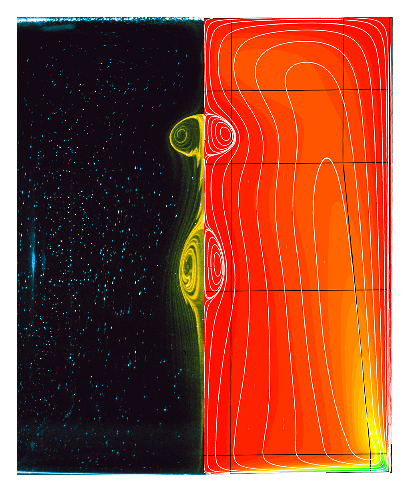
\includegraphics[width=0.5\textwidth]{vbmed_bitmap.eps}}
\end{center}
\end{figure}

\vspace{\fill}

{\large H.\,M. Blackburn}\\
Monash University

\vspace{\fill}

\today

\Semtex\ version 8.1

\vspace*{\fill}

\end{titlepage}

%%%%%%%%%%%%%%%%%%%%%%%%%%%%%%%%%%%%%%%%%%%%%%%%%%%%%%%%%%%%%%%%%%%%%%%%%%%%%%

\tableofcontents

\clearpage

%%%%%%%%%%%%%%%%%%%%%%%%%%%%%%%%%%%%%%%%%%%%%%%%%%%%%%%%%%%%%%%%%%%%%%%%%%%%%
\chapter{Introduction}

\Semtex\ is a family of spectral element simulation codes, most
prominently a code for direct numerical simulation of incompressible
flow.  The spectral element method is a high-order finite element
technique that combines the geometric flexibility of finite elements
with the high accuracy of spectral methods.  The method was pioneered
in the mid 1980's by Anthony Patera at MIT
\citep{pat84,kp86}. \Semtex\ uses parametrically mapped quadrilateral
elements, the classic GLL `nodal' shape function basis, and continuous
Galerkin projection.  Algorithmically the code is similar to Ron
Henderson's \emph{Prism} \citep{hk95,kh98,hen99b}, but with some
differences in design, and lacks mortar element capability. A notable
extension is that \Semtex\ can solve problems in cylindrical as well
as Cartesian coordinate systems \citep{blsh04}.

%-----------------------------------------------------------------------------
\section{Numerical method}

Some central features of the spectral element method are
\begin{description}
\item[Orthogonal polynomial-based shape functions] Spectral accuracy
is achieved by using tensor-product Lagrange interpolants within each
element, where the nodes of these shape functions are placed at the
zeros of Legendre polynomials mapped from the canonical domain
[-1,~1]$\times$[-1,~1] to each element.  In one spatial dimension, the
resulting Gauss--Lobatto--Legendre Lagrange interpolant which is unity
at one of the $N + 1$ Gauss--Lobatto points $x_j$ in [-1, 1] and zero at
the others is
\begin{equation}
\psi_j(x) = \frac{1}{N(N+1)L_N(x_j)}\frac{(1-x^2)L_N^\prime(x)}{x - x_j}.
\end{equation}
For example, the family of sixth-order GLL Lagrange interpolants is
shown in figure~\ref{fig:shapes}.
\begin{figure}

\begin{center}
  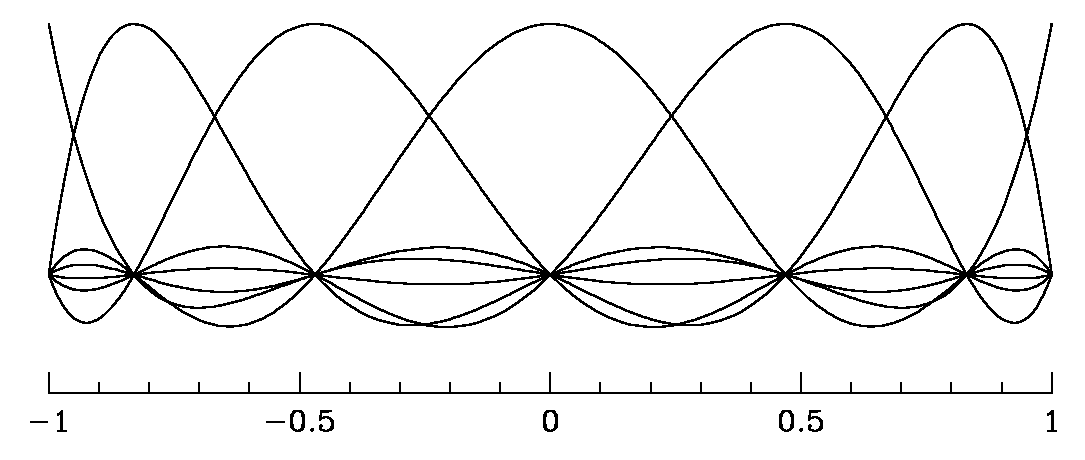
\includegraphics[width=0.5\textwidth]{shape7x7.eps}
\end{center}
\caption{The family of sixth-order one-dimensional GLL Lagrange shape
  functions on the master domain $[-1,+1]$.}
\label{fig:shapes}
\end{figure}
In smooth function spaces it can be shown that the resulting
interpolants converge exponentially fast (faster than any negative
integer power of $N$) as the order of the interpolant is increased.
See \citet{chqz88}, \S\S\,2.3.2 and~9.4.3.
\item[Gauss--Lobatto quadrature] Efficiency (particularly in iterative
  methods) is achieved by using Gauss--Lobatto quadrature for
  evaluating elemental integrals: the quadrature points reside at the
  nodal points, which enables fast tensor-product techniques to be
  used for iterative matrix solution methods.  Gauss--Lobatto
  quadrature on the nodal points delivers diagonal mass matrices.
\item[Static condensation]
Direct matrix solutions are sped up by using static condensation
coupled with bandwidth reduction algorithms to reduce storage
requirements for assembled system matrices.
\end{description}

While the numerical method is very accurate and efficient, it also has
the advantage that complex geometries can be accommodated by employing
unstructured meshes.  The vertices of spectral elements meshes can be
produced using finite-element mesh generation procedures, or any other
method (for \Semtex, only meshes with quadrilateral elements are
accepted).

Time integration employs a backwards-time differencing scheme
described by \citet{kio91}, more recently classified as a
velocity-correction method by \citet{gush03}. One can select first,
second, or third-order time integration, but second order is usually a
reasonable compromise, and is the default scheme. Equal-order
interpolation is used for velocity and pressure
\citep[see][]{gms06}. 

As of \Semtex~V8, the `alternating skew symmetric' form \citep{zan91b}
is the default for construction of nonlinear terms in the
\NavSto\ equations (faster and just as robust as full skew symmetric,
which is still an option), and no dealiasing of product terms is
carried out for either serial or parallel operations.  As an aid to
robust operation at high Reynolds numbers, `spectral vanishing
viscosity' \citep{xupa04} can easily be enabled by setting appropriate
control tokens.
%
A significant additional novelty of \Semtex~V8 is the option of robust
outflow boundary conditions \citep{dkc14}, which alleviate much of the
numerical stability problem associated with inflows that occur at the
outflow boundary.

%-----------------------------------------------------------------------------
\section{Implementation}

The top level of the code is written in C++, with calls to C and
FORTRAN library routines, \eg BLAS and LAPACK. The original
implementation for two-dimensional Cartesian geometries was extended
to three dimensions using Fourier expansion functions for
spatially-periodic directions in Cartesian and cylindrical spaces.
Concurrent execution is supported, using MPI as the basis for
interprocessor communications, and the code has been ported to DEC,
NEC, Fujitsu, Compaq, SGI, Apple and Linux multiprocessor
machines. Basically it ought to work with little trouble on any
contemporary UNIX system.

There are various code extensions that are not part of the base
distribution. These include dynamic and non-dynamic LES
\citep{blsc03}, simple power-law type non-Newtonian rheologies
\citep{rb06}, scalar transport \citep{hmb01a,hmb02b}, buoyancy via the
Boussinesq approximation, accelerating frame of reference coupling for
aeroelasticity \citep{bh96a,bh99,bgw01,hmb03}, solution of
steady-state flows via Newton--Raphson iteration \citep{hmb02a}

However, linear stability analysis
\citep{hmb02a,bllo03b,bllo03a,bml05,shbl05,ebs06,blsh07} and optimal
transient growth analysis \citep{bbs08a} are released as an additional
code base (called \Dog), see the accompanying user guide called
`Working \Dog'.

%-----------------------------------------------------------------------------
\section{Further reading}

The most comprehensive references on spectral methods in general are
\citet{gs77}, \citet{chqz88,chqz06}.  The first papers by
\citet{pat84} and \citet{kp86} provide a good introduction to spectral
elements, although some aspects have changed with time and
\citet{mt89} is more up-to-date.  The use of Fourier expansions to
extend the method to three spatial dimensions is discussed by
\citet{ap89}, \citet{kar89} and \citet{kar90}.  The use of spectral
element techniques in cylindrical coordinates is dealt with in
\citet{blsh04}.  The book by \citet{fun97} provides useful information
and further references.  Recent overviews and some applications appear
in \citet{kh98,hen99b}.  The definitive reference is now the book by
\citet{kars05}, but you will also find the text by \citet*{dfm02}
useful for alternative explanations and views. More recently, the book
by \citet{chqz07} provides both theory and applications of spectral as
well as spectral element methods in fluid dynamics.

%%%%%%%%%%%%%%%%%%%%%%%%%%%%%%%%%%%%%%%%%%%%%%%%%%%%%%%%%%%%%%%%%%%%%%%%%%%%%
\chapter{Starting out}

It is assumed you're using some version of UNIX (which includes Mac OS
X), and the current \Semtex\ versions assume that your C++ compiler
supports the standard libraries. Makefiles assume GNUmake (by now this
is usually the standard supplied variant of \texttt{make}).
\SM\ and \emph{Tecplot} would be nice to have but are not
essential to get up and running, and VTK-based post processors such as
\emph{VisIt} or \emph{ParaView} can alternatively be used for
post-processing in place of \emph{Tecplot}. All major executables have
a \texttt{-h} command line option which provides a usage prompt.

Application programs/Makefiles can be found in top and upper-level
directories:
\begin{tabbing}
\texttt{ellipticxx} \= \kill
\texttt{elliptic} \> Solve elliptic (Laplace, Poisson, Helmholtz)
problems.\\ \texttt{dns} \> Solve time-varying incompressible
\NavSto\ problems, Cartesian/cylindrical.
\end{tabbing}

%============================================================================
\section{Testing}

Unpack the tar file, then run \texttt{make test}. This will copy
header files to their correct places, compile and place the libraries,
make two central utilities (\texttt{compare} and \texttt{enumerate}),
then make the direct numerical simulation solver \texttt{dns} and run
regression checks on its output for a number of test cases. If all
goes well, this process will end with a number of tests reported as
\texttt{passed}. In that case, go on and compile all the utilities,
too (\texttt{cd utility; make all}).

%----------------------------------------------------------------------------
\subsection{Troubleshooting installation problems}
If the above process didn't work, there are a number of possible
things lacking on your system, e.g.:
\begin{enumerate}
\item GNU's \texttt{make}: it needs to be in your \texttt{path}
  somewhere.  On most current UNIX systems, the system-supplied
  \texttt{make} \emph{is} the GNU version. So now (as of 2010) this is
  assumed; you can easily check by running \texttt{make --version} and
  looking at the first line of output.  If not, it may be installed as
  \texttt{gmake}. Otherwise you will need to get it installed. Alter
  the variable \texttt{MAKE} in \texttt{semtex/Makefile} so that it
  gets to the installed GNU \texttt{make}, if required.
\item The BLAS and LAPACK libraries\,---\,these may be in
  \texttt{/usr/lib} or \texttt{/usr/local/lib}: search for
  \texttt{libblas} and \texttt{liblapack}.  On many systems, BLAS and
  LAPACK are vendor-supplied as part of some `math kernel' library.
  NB: since quite heavy use is made of BLAS routine \texttt{dgemm}, it
  can be worthwhile finding BLAS versions in which this is well
  optimised, see \S\,\ref{sec.speed}.
\item A standard C++ compiler, a C compiler, and a FORTRAN compiler
  that can deal with FORTRAN-77.  Note that F90, F95 compilers now
  often supplant F77 compilers, and these can (and should) be
  substituted if available. GNU's standard FORTRAN compiler is now
  called \texttt{gfortran} and is part of the standard \texttt{gcc}
  compiler suite.
\end{enumerate}
If you have all these things but there are still compilation problems,
you have some work to do.

The first place to look is in the file \texttt{src/Makefile} which has
the master set of compilation flags and directives for various
operating systems. You my find your system here, or one that is
similar. Even if this is not the case, you should pick up some clues
about how to set up for compilation on a new system.  As well, check
the \texttt{README} file in the top directory. Of course, it is
possible that the code is incompatible with some detail of your
compilation system or has a bug, but it has had fairly extensive
exercise on a number of UNIX systems by now. 

If you are having problems, it's usually best to start small and work
up. First try to make and install the \verb+veclib+ and \verb+femlib+
libraries, since they do not use C++ or the linker. Try
\verb+make libs+ at the top level, then if this is still problematic
go to the \verb+veclib+ directory, do \texttt{make clean; make; make
install}. When that works, do the same in the \texttt{femlib}
directory. Next move on and try a simple C++ compile and link, e.g.\
in the \texttt{utility} directory do \texttt{make calc} and try
running \texttt{calc} (which is a little like the UNIX calculator
utility \texttt{bc}, but uses \Semtex's function parser, and links
\texttt{libfem.a}, the library produced in \texttt{femlib}): try say
\texttt{1+1}. Next you should try compiling something that links to
the BLAS and LAPACK, e.g.\ \texttt{compare}. Once this will compile,
everything should.


%============================================================================
\section{Files}

\Semtex\ uses a base input file which describes the mesh, boundary
conditions.  We call this a \verb+session+ file and typically it has
no root extension.  It is written in a format patterned on HTML, which
we have called FEML (for Finite Element Markup Language).  There are a
number of example session files in the mesh directory.  Other files
have standard extensions:
\begin{tabbing}
\texttt{session.numxx} \= \kill
\texttt{session.num}  \>
        Global node numbers, produced by enumerate utility.\\
\texttt{session.fld}  \>
        Solution/field file.  Binary format by default.\\
\texttt{session.rst}  \>
        Restart file. Read in to initialize solution if present.\\
\texttt{session.avg} \> Averaged results. Read back in for
        continuation (over-written).\\
\texttt{session.his} \> History point data.\\
\texttt{session.flx} \> Time series of pressure and viscous forces
        integrated over the \texttt{wall} boundary group.\\
\texttt{session.mdl} \> Time series of kinetic energies in the Fourier modes.\\
\texttt{session.par} \> Used to define initial particle locations.\\
\texttt{session.trk} \> Integrated particle locations.\\
\end{tabbing}
When writing a new session file it is best to run \texttt{meshpr}
(and/or \texttt{meshpr -c}) on it before trying to use it for
simulations.  \texttt{Meshpr} will catch most of the easier-to-make
errors.  You can also plot up the results using \SM\ or other
utility as a visual check.

%============================================================================
\section{Utilities}

Source code for these is found in the \texttt{utility} directory. You
will need to make most of these by hand (using the supplied
\texttt{Makefile}, and \texttt{make all}).  Here is a summary:
\begin{tabbing}
\texttt{enumeratexx}  \= \kill
\texttt{addfield} \>   
        Add vorticity vector components, divergence, etc., to a field
	file.\\
\texttt{calc} \>      
        A simple calculator that calls \verb+femlib+'s function
        parser. The default functions\\\>and \texttt{TOKENS} can be seen
        if you run \texttt{calc -h}.\\
\texttt{compare} \>   
        Generate restart files, compare solutions to a function.\\
\texttt{convert} \>   
        Convert field file formats (IEEE-big/little, ASCII).\\
\texttt{eneq} \>   
        Compute terms in the energy transport equation.\\
\texttt{enumerate}  \>
        Generate global node numbering, with RCM optimization.\\
\texttt{integral} \> Obtain the 2D integral of fields over the
        domain area.\\
\texttt{interp} \>   
        Interpolate a field file onto a (2D) set of points.\\
\texttt{meshpr} \>    
        Generate 2D mesh locations for plotting or checking.\\
\texttt{noiz} \>      
        Add a random perturbation to a field file.\\
\texttt{probe} \>   
        Probe a field file at a set of 2D/3D points. Different
        interfaces to \texttt{probe}\\ \> are obtained through the names
        \texttt{probeline} and \texttt{probeplane}: \\ \> make these soft
        links by hand.\\
\texttt{project} \>   
        Convert a field file to a different order interpolation.\\
\texttt{rectmesh} \>
        Generate a template session file for a rectangular domain.\\
\texttt{resubmit} \> Shell utility for automatic job resubmission.\\
\texttt{rstress} \>
	Postprocess to compute Reynolds stresses from a file of
        time-averaged variables.\\
\texttt{save} \> Shell utility for automatic job resubmission.\\
\texttt{sem2tec} \>   
        Convert field files to Amtec \emph{Tecplot} format.\\
        \> Note that by default, \verb|sem2tec| interpolates the original GLL-        mesh-based data onto \\
        \> a (isoparametrically mapped) uniform mesh for improved visual 
        appearance.  Sometimes\\ \>  it is useful to see the original data 
        (and mesh); for this use the \verb+-n 0+ command-line \\ 
         \> argument to \verb+sem2tec+.\\
\texttt{sem2vtk} \>   
        Convert field files to VTK format (\emph{VisIt, ParaView}).\\
\texttt{transform} \>      
        Take Fourier, Legendre, modal basis transform of a field
	file. Invertible.\\
\texttt{wallmesh} \>      
        Extract the mesh nodes corresponding to surfaces with the
	\verb+wall+ group.
\end{tabbing}


%%%%%%%%%%%%%%%%%%%%%%%%%%%%%%%%%%%%%%%%%%%%%%%%%%%%%%%%%%%%%%%%%%%%%%%%%%%%%
\chapter{Examples and hints}

We will run through some examples to illustrate input files, utility
routines, and the use of the solvers.

%============================================================================
\section{2D Taylor flow}

Taylor flow is an analytical solution to the \NavSto\ equations.
In the $x$--$y$ plane the solution is 
\begin{eqnarray}
        u &=& -\cos(\pi x) \sin(\pi y) \exp(-2\pi^2\nu t),\\
        v &=& +\sin(\pi x) \cos(\pi y) \exp(-2\pi^2\nu t),\\
        p &=& -(\cos(2\pi x) + \cos(2\pi y)) \exp(-4\pi^2\nu t)/4.
\end{eqnarray}
The solution is doubly periodic in space, with periodic length 2.  As
usual for \NavSto\ solutions, the pressure can only be specified
up to an arbitrary constant.  An interesting feature of this solution
is that the nonlinear and pressure gradient terms balance one another,
leaving a diffusive decay of the initial condition --- this property
is occasionally useful for checking codes.

%----------------------------------------------------------------------------
\subsection{Session file}

Below is the complete input or \emph{session} file we will use; it
has four elements, each of the same size, with 11 nodes along each
edge.  We will call this session file \texttt{taylor2} in the
following.

{\small
\begin{verbatim}
##############################################################################
# 2D Taylor flow in the x--y plane has the exact solution
#
#       u = -cos(PI*x)*sin(PI*y)*exp(-2.0*PI*PI*KINVIS*t)
#       v =  sin(PI*x)*cos(PI*y)*exp(-2.0*PI*PI*KINVIS*t)
#       w =  0
#       p = -0.25*(cos(2.0*PI*x)+cos(2.0*PI*y))*exp(-4.0*PI*PI*KINVIS*t)
#
# Use periodic boundaries (no BCs).

<USER>
        u = -cos(PI*x)*sin(PI*y)*exp(-2.0*PI*PI*KINVIS*t)
        v =  sin(PI*x)*cos(PI*y)*exp(-2.0*PI*PI*KINVIS*t)
        p = -0.25*(cos(TWOPI*x)+cos(TWOPI*y))*exp(-4.0*PI*PI*KINVIS*t)
</USER>

<FIELDS>
        u v p
</FIELDS>

<TOKENS>
        N_TIME  = 2
        N_P     = 11
        N_STEP  = 20
        D_T     = 0.02
        Re      = 100.0
        KINVIS  = 1.0/Re
        TOL_REL = 1e-12
</TOKENS>

<NODES NUMBER=9>
        1       0.0       0.0       0.0
        2       1.0       0.0       0.0
        3       2.0       0.0       0.0
        4       0.0       1.0       0.0
        5       1.0       1.0       0.0
        6       2.0       1.0       0.0
        7       0.0       2.0       0.0
        8       1.0       2.0       0.0
        9       2.0       2.0       0.0
</NODES>

<ELEMENTS NUMBER=4>
        1 <Q> 1 2 5 4 </Q>
        2 <Q> 2 3 6 5 </Q>
        3 <Q> 4 5 8 7 </Q>
        4 <Q> 5 6 9 8 </Q>
</ELEMENTS>

<SURFACES NUMBER=4>
        1       1       1       <P>     3       3       </P>
        2       2       1       <P>     4       3       </P>
        3       2       2       <P>     1       4       </P>
        4       4       2       <P>     3       4       </P>
</SURFACES>
\end{verbatim}
}

The first section of the file in this case contains comments; a line
anywhere in the session file which starts with a \verb+#+ is
considered to be a comment.  Following that are a number of sections
which are opened and closed with matching keywords in HTML style (e.g.
\verb+<USER>+--\verb+<\USER>+).  Keywords are not case sensitive.
The complete list of keywords is: \texttt{TOKENS}, \texttt{FIELDS}, 
\texttt{GROUPS}, \texttt{BCS}, \texttt{NODES}, \texttt{ELEMENTS}, 
\texttt{SURFACES}, \texttt{CURVES} and \texttt{USER}.  Depending on the
problem being solved, some sections may not be needed, but the minimal
set is: \texttt{FIELDS}, \texttt{NODES}, \texttt{ELEMENTS} and
\texttt{SURFACES}.  Anywhere there is likely to be a long list of
inputs within the sections, the \texttt{NUMBER} of inputs is also
required; this currently applies to \texttt{GROUPS}, \texttt{BCS},
\texttt{NODES}, \texttt{ELEMENTS}, \texttt{SURFACES} and
\texttt{CURVES}.  In each of these cases the numeric tag appears first for
each input, which is free-format.  The order in which the sections
appear in the session file is irrelevant.

The \texttt{USER} section is ignored by the solvers, and is used
instead by utilities --- in this case it will be used by the
\texttt{compare} utility both to generate the initial condition or
\emph{restart} file and to check the computed solution.  This
section declares the variables corresponding to the solution fields
with the corresponding analytical solutions.  The variables
\texttt{x}, \texttt{y}, \texttt{z} and \texttt{t} can be used to
represent the three spatial coordinates and time.  Note that some
constants such as \texttt{PI} and \texttt{TWOPI} are predefined, while
others, like \texttt{KINVIS}, are set in the \texttt{TOKENS} section.
Note also the use of predefined functions, accessed through an inbuilt
function parser\footnote{The built-in functions and predefined constants
can be found by running \texttt{calc -h}.}.

The \texttt{FIELDS} section declares the one-character names of
solution fields.  The names are significant: \texttt{u}, \texttt{v}
and \texttt{w} are the three velocity components (we only use
\texttt{u} and \texttt{v} here for a 2D solution and the \texttt{w}
component is always the direction of Fourier expansions), \texttt{p}
is the pressure field.  The field name \texttt{c} is also recognized
as a scalar field for certain solvers, e.g. the elliptic solver.

In the \texttt{TOKENS} section, second-order accurate time integration
is selected (\verb+N_TIME = 2+) and the number of Lagrange knot points
along the side of each element is set to 11 (\verb+N_P = 11+).  The
code will integrate for 20 timesteps (\verb+N_STEP = 20+) with a
timestep of 0.02 (\verb+D_T = 0.002+).  The kinematic viscosity is
set as the inverse of the Reynolds number (100): note the use of the
function parser here.  Finally the relative tolerance used as a
stopping test in the PCG iteration used to solve the viscous substep
on the first timestep is set as $1.0\times10^{-12}$.

The shape of the mesh is defined by the \texttt{NODES} and
\texttt{ELEMENTS} sections.  Here there are four elements, each
obtained by connecting the corner nodes in a counterclockwise
traverse.  The $x$, $y$ and $z$ locations of the nodes are given, and
the four numbers given for the nodes of each element are indices
within the list of nodes.

In the final section (\texttt{SURFACES}), we describe how the edges of
elements which define the boundary of the solution domain are dealt
with.  In this example, the solution domain is periodic and there are
no boundary conditions to be applied, so the \texttt{SURFACES} section
describes only periodic (\verb+P+) connections between elements.  For
example, on the first line, side~1 of element~1 is declared to be
periodic with side~3 of element~3 --- side~1 runs between the first
and second nodes, while side~3 runs between the third and fourth.

%----------------------------------------------------------------------------
\subsection{Running the codes}

Assume we're in the \texttt{dns} directory of the distribution, that
the \texttt{enumerate}, \texttt{compare}, \texttt{meshpr} and
\texttt{sem2tec} utilities have been compiled, as well as the
\texttt{dns} simulation code.
{\small
\begin{verbatim}
karman[16] cp ../mesh/taylor2 .
\end{verbatim}
}

First we'll examine the mesh, using \SM\ macros.
{\small
\begin{verbatim}
karman[17] meshpr taylor2 > taylor2.msh
karman[18] sm
Hello Hugh, please give me a command
: meshplot taylor2.msh 1
Read lines 1 to 1 from taylor2.msh
Read lines 2 to 485 from taylor2.msh
: meshnum
: meshbox
: quit
\end{verbatim}
}
\noindent
You should have seen a plot like that in figure~\ref{tay2msh}. (Note:
while you are building up the mesh parts of a session file, you can
use \texttt{meshpr -c} to suppress some of the checking for matching
element edges and curved boundaries that \texttt{meshpr} does by
default.)
\begin{figure}
\begin{center}
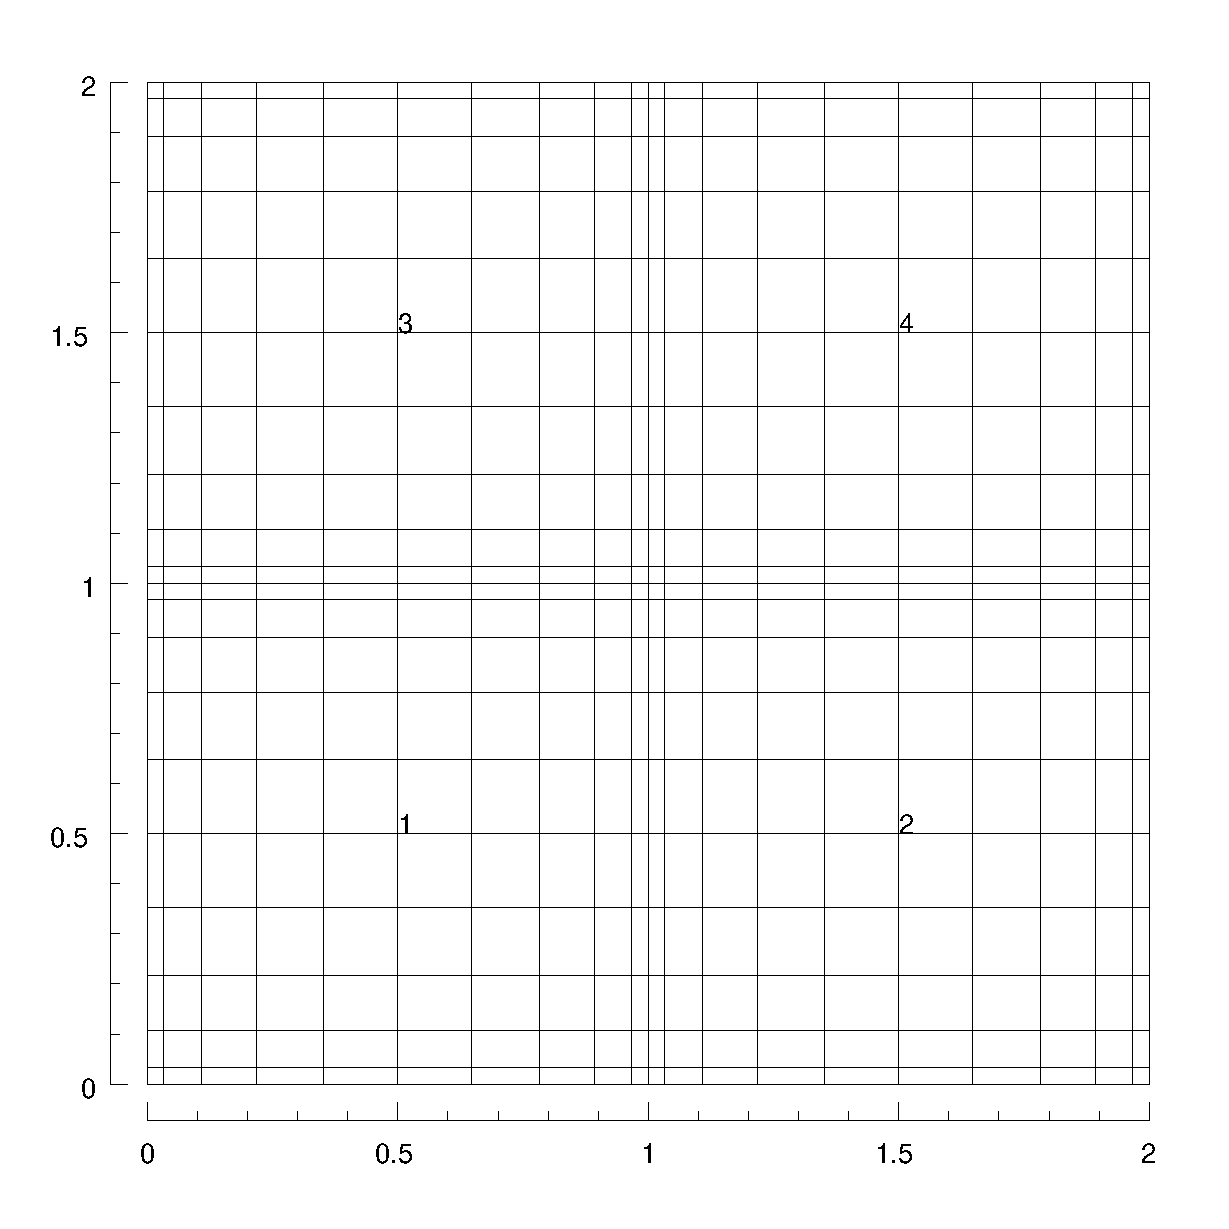
\includegraphics[width=0.5\textwidth]{taylor2mesh.eps}
\end{center}
\caption{
\label{tay2msh}
  The mesh corresponding to the \texttt{taylor2} session file.
}
\end{figure}

Next we will generate the global numbering schemes for the solution
using \texttt{enumerate} to produce \texttt{taylor2.num}.  The
solution code would run \texttt{enumerate} automatically to generate
\texttt{taylor2.num} if it were not present, but we will run it `by
hand' to highlight its existence and illustrate its use.
{\small
\begin{verbatim}
karman[19] enumerate taylor2 > taylor2.num
karman[20] head -20 taylor2.num
# FIELDS         :  uvp
# ----------------  ----------
# 1 NUMBER SETS  :         uvp
# NEL            :           4
# NP_MAX         :          11
# NEXT_MAX       :          40
# NINT_MAX       :          81
# NTOTAL         :         484
# NBOUNDARY      :         160
# NGLOBAL        :          76
# NSOLVE         :          76
# OPTIMIZATION   :           1
# BANDWIDTH      :          67
# ----------------  ----------
# elmt  side offst  bmap  mask
     1     1     0    20     0
     1     1     1    17     0
     1     1     2    16     0
     1     1     3    15     0
     1     1     4    14     0
\end{verbatim}
}

The \texttt{compare} utility is used to generate a file of initial
conditions using information in the \verb|USER| section of a session
file.  This \emph{restart} file contains binary data, but we'll have a
look at the start of it by converting it to ASCII format.  Also, the
header of these files is always in ASCII format, and so can be
examined directly using the Unix \texttt{head} command.  {\small
\begin{verbatim}
karman[21] compare taylor2 > taylor2.rst
karman[22] convert taylor2.rst | head -20
taylor2                   Session
Wed Aug 13 21:39:47 1997  Created
11   11   1    4          Nr, Ns, Nz, Elements
0                         Step
0                         Time
0.02                      Time step
0.01                      Kinvis
1                         Beta
uvp                       Fields written
ASCII                     Format
     0.000000000      0.000000000    -0.5000000000 
     0.000000000     0.1034847104    -0.4946454574 
     0.000000000     0.3321033052    -0.4448536974 
     0.000000000     0.6310660897    -0.3008777952 
     0.000000000     0.8940117093    -0.1003715318 
     0.000000000      1.000000000      0.000000000 
     0.000000000     0.8940117093    -0.1003715318 
     0.000000000     0.6310660897    -0.3008777952 
     0.000000000     0.3321033052    -0.4448536974 
     0.000000000     0.1034847104    -0.4946454574 
\end{verbatim}
}

Then the \texttt{dns} solver is run to generate a solution or
\emph{field} file, \texttt{taylor2.fld}.  This has the same format
as the restart file.
{\small
\begin{verbatim}
karman[23] dns taylor2
-- Restarting from file:  taylor2.rst
   Start time       : 0
   Time step        : 0.02
   Number of steps  : 20
   End time         : 0.4
   Integration order: 2
-- Building matrices for Fields "uvp"   [*]
-- Building matrices for Fields "uvp"   [.]
-- Building matrices for Fields "uvp"   [*]
Step: 1  Time: 0.02
Step: 2  Time: 0.04
Step: 3  Time: 0.06
Step: 4  Time: 0.08
Step: 5  Time: 0.1
Step: 6  Time: 0.12
Step: 7  Time: 0.14
Step: 8  Time: 0.16
Step: 9  Time: 0.18
Step: 10  Time: 0.2
Step: 11  Time: 0.22
Step: 12  Time: 0.24
Step: 13  Time: 0.26
Step: 14  Time: 0.28
Step: 15  Time: 0.3
Step: 16  Time: 0.32
Step: 17  Time: 0.34
Step: 18  Time: 0.36
Step: 19  Time: 0.38
Step: 20  Time: 0.4
\end{verbatim}
}

We can use \texttt{compare} to examine how close the solution is to the
analytical solution.  The output of \texttt{compare} in this case
is a field file which contains the difference: since we're only interested
in seeing error norms here, we'll discard this field file.
{\small
\begin{verbatim}
karman[24] compare taylor2 taylor2.fld > /dev/null
Field 'u': norm_inf: 1.13019e-05
Field 'v': norm_inf: 1.13019e-05
Field 'p': norm_inf: 0.422391
\end{verbatim}
}
\noindent
The velocity error norms are small, as expected, but the pressure norm
will always be arbitrary, corresponding to the fact that the pressure
can only be specified to within an arbitrary constant.

Finally we will use \texttt{sem2tec} to generate a \emph{Tecplot}
input file.  The \emph{Tecplot} utility \texttt{preplot} must also be
in your \texttt{path}.  {\small
\begin{verbatim}
karman[36] sem2tec -m taylor2.msh taylor2.fld
\end{verbatim}
}
\noindent
This produces \texttt{taylor2.plt} which can be used as input to
\texttt{tecplot}.  The plot in figure~\ref{tay2soln} was generated
using \texttt{tecplot} and shows pressure contours and velocity
vectors.  Notice that by default \texttt{sem2tec} interpolates the
results from the Gauss--Lobatto--Legendre grid (seen in
figure~\ref{tay2msh}) used in the computation to a uniformly-spaced
grid of the same order (use \verb|-n 0| to disable this feature).
\begin{figure}
\begin{center}
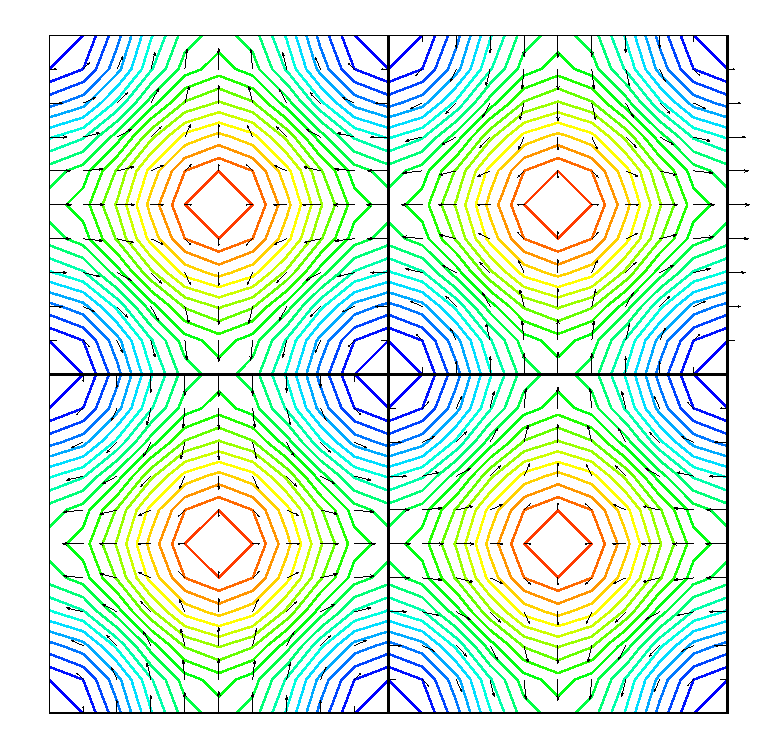
\includegraphics[width=0.5\textwidth]{taylor2.eps}
\end{center}
\caption{
\label{tay2soln}
  Solution to the \texttt{taylor2} problem, visualized using \emph{Tecplot}.
}
\end{figure}

%============================================================================
\section{2D Laplace problem}
\label{sec.laplace}

In this section we illustrate the use of the elliptic solver for a 2D
Laplace problem, $\nabla^2 c = 0$.  In this case the function
\begin{equation}
  c(x,y) = \sin(x) \exp(-y)
\end{equation}
satisfies Laplace's equation and is used to set the boundary
conditions.  This example illustrates the methods used to set BCs and
also to generate curved element boundaries.  Also we will demonstrate
the selection of the PCG solver.  We will call the session file
\texttt{laplace6}.

The elliptic solver can also be used to solve Poisson and Helmholtz
problems in 2D and 3D Cartesian and cylindrical coordinate systems.
Apart from this use it provides a means to test new formulations of
elliptic solution routines used also in the \NavSto\ type
solvers.

{\small
\begin{verbatim}
##############################################################################
# Laplace problem on unit square, BC c(x, y) = sin(x)*exp(-y)
# is also the analytical solution.  Use essential (Dirichlet) BC
# on upper, curved edge, with natural (Neumann) BCs elsewhere.

<FIELDS>
        c
</FIELDS>

<USER>
        c =  sin(x)*exp(-y)
</USER>

<TOKENS>
        N_P      = 11
        TOL_REL  = 1e-12
        STEP_MAX = 1000
</TOKENS>

<GROUPS NUMBER=4>
        1       d       value
        2       a       slope
        3       b       slope
        4       c       slope
</GROUPS>

<BCS NUMBER=4>
        1       d       1
                        <D>     c =  sin(x)*exp(-y)     </D>
        2       a       1
                        <N>     c = -cos(x)*exp(-y)     </N>
        3       b       1
                        <N>     c =  cos(x)*exp(-y)     </N>
        4       c       1
                        <N>     c =  sin(x)*exp(-y)     </N>
</BCS>

<NODES NUMBER=9>
        1       0.0     0.0     0.0
        2       0.5     0.0     0.0
        3       1.0     0.0     0.0
        4       0.0     0.5     0.0
        5       0.5     0.5     0.0
        6       1.0     0.5     0.0
        7       0.0     1.0     0.0
        8       0.5     1.0     0.0
        9       1.0     1.0     0.0
</NODES>

<ELEMENTS NUMBER=4>
        1       <Q>     1 2 5 4         </Q>
        2       <Q>     2 3 6 5         </Q>
        3       <Q>     4 5 8 7         </Q>
        4       <Q>     5 6 9 8         </Q>
</ELEMENTS>

<SURFACES NUMBER=8>
        1       1       1       <B>     c       </B>
        2       2       1       <B>     c       </B>
        3       2       2       <B>     b       </B>
        4       4       2       <B>     b       </B>
        5       4       3       <B>     d       </B>
        6       3       3       <B>     d       </B>
        7       3       4       <B>     a       </B>
        8       1       4       <B>     a       </B>
</SURFACES>

<CURVES NUMBER=1>
        1       4       3       <ARC>   1.0     </ARC>
</CURVES>
\end{verbatim}
}

%----------------------------------------------------------------------------
\subsection{Curved element edges}

The mesh is somewhat similar to that for the Taylor flow example, the
only difference being in the use of a curved edge for the 3rd edge of
element~4, as specified in the \texttt{CURVES} section.  Both
\texttt{ARC} and \texttt{SPLINE} type curves are currently
implemented.  For the \texttt{ARC} type, the parameter supplies the
radius of the curve: a positive value implies that the curve makes the
element convex on that side, while a negative value implies a concave
side.  Note that where elements mate along a curved side, the curve
must be defined twice, once for each element, and with radii of
different signs on each side.  The mesh for this problem can be seen
in figure~\ref{lapcurve}.

\begin{figure}
\begin{center}
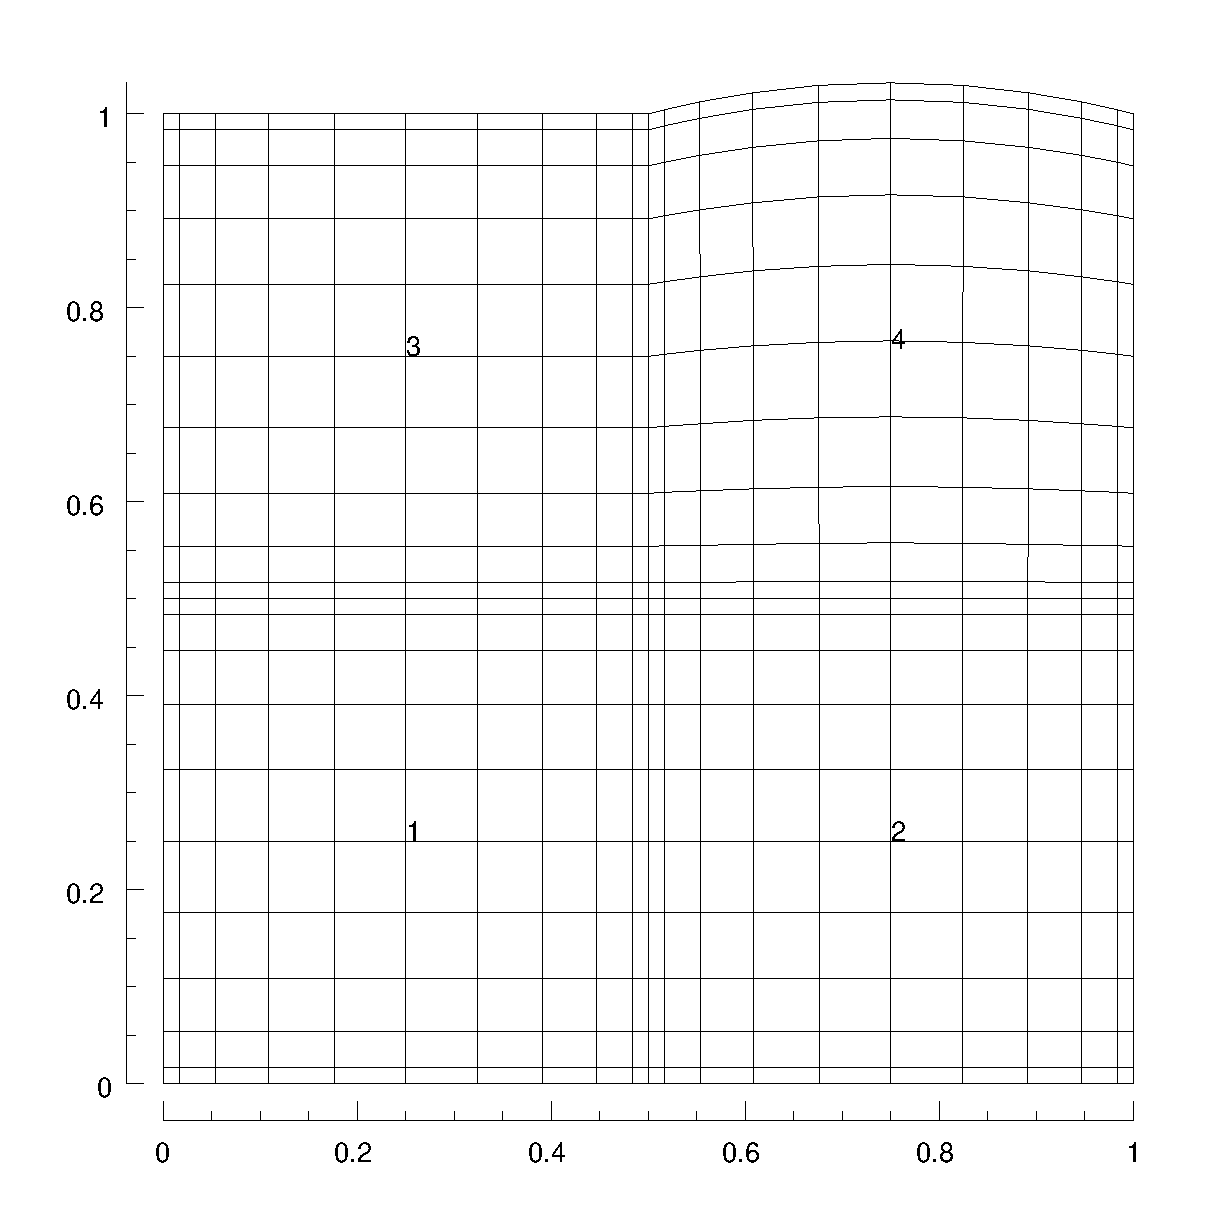
\includegraphics[width=0.5\textwidth]{laplace6mesh.eps}
\end{center}
\caption{
\label{lapcurve}
  The mesh corresponding to the \texttt{laplace6} session file.
}
\end{figure}

For the \texttt{SPLINE} type, the parameter supplies the name of an
ASCII file which contains a list of ($x$,\,$y$) coordinate pairs
(white-space delimited). Naturally, the list of points should be in
arc-length order. A single file can be used to supply the curved edges
for a set of element edges. The vertices of the relevant elements do
not have to lie exactly on the splined curve\,---\,if they do not,
those vertices get shifted to the intersection of the projection of
the straight line joining the original vertex position and its
neighbouring ``curve-normal' vertex, and the cubic spline joining the
points in the file. On the other hand, it is good practise to ensure
that the declared vertex locations lie close to the spline, and to
check the mesh that is produced: use \texttt{meshpr} to do this.

%----------------------------------------------------------------------------
\subsection{Boundary conditions}

The other new sections introduced in the session file for this example
(\texttt{GROUPS}, \texttt{BCS}) are used to impose boundary conditions
on the problem.  The \texttt{GROUPS} section associates a character
group tag (\eg \verb+d+) with a string (\eg \verb+value+), but note
that different groups can be associated with the same
string\footnote{This allows actions to be taken over a set of BCs
  which share the same string.}.  Groups \verb+a+, \verb+b+ and
\verb+c+ will be used to set natural (\ie slope or Neumann), boundary
conditions ($\partial c/\partial n=\textrm{value}$), while group
\verb+a+ will be used to impose an essential or Dirichlet condition
($c=\textrm{value}$).

The \texttt{BCS} section is used to define the boundary conditions
which will be applied for each group.  For each group, after the
numeric tag (ignored) appears the character for that group, then the
number of BCs that will be applied: this corresponds to the number of
fields in the problem, in this case~1 (\verb+c+).  BCs are typically
of Dirichlet, Neumann, or mixed type (note that domain periodicity can
be employed but that this does not constitute a boundary condition).
So in this case we will declare the BC types to be \verb+D+ ({\texttt
  D}irichlet) for group \verb+d+ and \verb+N+ ({\texttt N}eumann) for
groups \verb+a+, \verb+b+ and \verb+c+.  On Neumann boundaries, the
value which must be supplied is the slope of the solution along the
outward normal to the solution domain.  Note the fact that the BCs can
be set using the function parser, using the built-in functions and
variables, also any symbols defined in the \texttt{TOKENS} section, as
well as the spatial variables \verb+x+, \verb+y+ and \verb+z+.  The
BCs can also be functions of time, \verb+t+, and for time-varying
problems the boundary conditions are re-evaluated every time step.

The BC groups are associated with element edges in the \texttt{SURFACES}
section, in a similar way to the use of periodic boundaries for the
\texttt{taylor2} problem, although the edges are set to be \verb+B+ (BC)
rather than \verb+P+ (periodic).

Periodic edges, Dirichlet, Neumann and mixed boundary conditions can
be arbitrarily combined in a problem.  Dirichlet conditions over-ride
Neumann ones where they meet (say at the corner node of an
element). See further discussion on boundary conditions in
\S\,\ref{sec.bcs} below.

%----------------------------------------------------------------------------
\subsection{Running the codes}

We will run the solver and compare the computed solution to the
analytical solution.  We will select the iterative (PCG) solver using
the \verb+-i+ command-line option to \texttt{elliptic}, then check the 
result using \texttt{compare}.
{\small
\begin{verbatim}
karman[287] elliptic -i laplace6
-- Initializing solution with zero IC
   Start time       : 0
   Time step        : 0.01
   Number of steps  : 1
   End time         : 0.01
   Integration order: 2
karman[288] compare laplace6 laplace6.fld > /dev/null
Field 'c': norm_inf: 1.37112e-08
\end{verbatim}
}

Next try the direct solver (default):
{\small
\begin{verbatim}
karman[288] compare laplace6 laplace6.fld > /dev/null
Field 'c': norm_inf: 1.37112e-08
karman[289] elliptic laplace6
-- Initializing solution with zero IC
   Start time       : 0
   Time step        : 0.01
   Number of steps  : 1
   End time         : 0.01
   Integration order: 2
-- Building matrices for Fields "c"     [*]
karman[290] compare laplace6 laplace6.fld > /dev/null
Field 'c': norm_inf: 3.10862e-15
\end{verbatim}
}
\noindent
In this case the direct solver is more accurate, but comparable
accuracy with the iterative solver could be obtained by decreasing
\verb+TOL_REL+ in the \texttt{TOKENS} section (and further increasing
\verb+STEP_MAX+, which has a default value of 500).

%============================================================================
\section{3D Kovasznay flow}
\label{sec.kovas}

Here we will solve another viscous flow for which an analytical
solution exists, the Kovasznay flow (we will call the session file
\verb+kovas3+).  In the $x$--$y$ plane, this flow is
\begin{eqnarray}
        u &=& 1 - \exp(\lambda x)\cos(2\pi y)           \\
        v &=& \lambda/(2\pi)\exp(\lambda x)\sin(2\pi y) \\
        w &=& 0                                         \\
        p &=& (1 - \exp(\lambda x))/2   
\end{eqnarray}
where $\lambda = \Rey/2 - (0.25\Rey^2 + 4\pi^2)^{1/2}$.

Although the solution has only two velocity components, we will set up
and solve the problem in three dimensions, with a periodic length in
the~$z$ direction of~1.0 and 8~$z$ planes of data.  The length in the
$z$ direction is set within the code by the variable \verb+BETA+ where
$\beta=2\pi/L_z$.  The default value of \verb+BETA+ is 1, so we reset
this in the \texttt{TOKENS} section using the function parser.  The
exact velocity boundary conditions are supplied on at the left and
right edges of the domain, and periodic boundaries are used on the
upper and lower edges (the domain has $-0.5\le y\le0.5$).  Since the
flow evolves to a steady state, first order timestepping is employed
(\verb+N_TIME = 1+).

{\small
\begin{verbatim}
##############################################################################
# Kovasznay flow in the x--y plane has the exact solution
#
#       u = 1 - exp(lambda*x)*cos(2*PI*y)
#       v = lambda/(2*PI)*exp(lambda*x)*sin(2*PI*y)
#       w = 0
#       p = (1 - exp(lambda*x))/2
#
# where lambda = Re/2 - sqrt(0.25*Re*Re + 4*PI*PI).
#
# This 3D version uses symmetry planes on the upper and lower boundaries
# with flow in the x-y plane.
#
# Solution accuracy is independent of N_Z since all flow is in the x--y plane.

<USER>
        u = 1.0-exp(LAMBDA*x)*cos(TWOPI*y)
        v = LAMBDA/(TWOPI)*exp(LAMBDA*x)*sin(TWOPI*y)
        w = 0.0
        p = 0.5*(1.0-exp(LAMBDA*x))
</USER>

<FIELDS>
        u v w p
</FIELDS>

<TOKENS>
        N_Z    = 8
        N_TIME = 1
        N_P    = 8
        N_STEP = 500
        D_T    = 0.008
        Re     = 40.0
        KINVIS = 1.0/Re
        LAMBDA = Re/2.0-sqrt(0.25*Re*Re+4.0*PI*PI)
        Lz     = 1.0
        BETA   = TWOPI/Lz
</TOKENS>

<GROUPS NUMBER=1>
        1       v       velocity
</GROUPS>

<BCS NUMBER=1>
        1       v       4
                        <D> u = 1-exp(LAMBDA*x)*cos(2*PI*y)             </D>
                        <D> v = LAMBDA/(2*PI)*exp(LAMBDA*x)*sin(2*PI*y) </D>
                        <D> w = 0.0                                     </D>
                        <H> p                                           </H>
</BCS>

<NODES NUMBER=9>
        1      -0.5    -0.5     0.0
        2       0      -0.5     0.0
        3       1      -0.5     0.0
        4      -0.5     0       0.0
        5       0       0       0.0
        6       1       0       0.0
        7      -0.5     0.5     0.0
        8       0       0.5     0.0
        9       1       0.5     0.0
</NODES>

<ELEMENTS NUMBER=4>
        1 <Q> 1 2 5 4 </Q>
        2 <Q> 2 3 6 5 </Q>
        3 <Q> 4 5 8 7 </Q>
        4 <Q> 5 6 9 8 </Q>
</ELEMENTS>

<SURFACES NUMBER=6>
        1       1       1       <P>     3       3       </P>
        2       2       1       <P>     4       3       </P>
        3       2       2       <B>     v               </B>
        4       4       2       <B>     v               </B>
        5       3       4       <B>     v               </B>
        6       1       4       <B>     v               </B>
</SURFACES>
\end{verbatim}
}

%----------------------------------------------------------------------------
\subsection{`High-order' pressure boundary condition}

Note that there is only one boundary group, and four boundary
conditions must be set, corresponding to the four fields \verb+u+,
\verb+v+, \verb+w+ and \verb+p+.  A new feature is a pressure BC of
type \verb+H+, which is an internally-computed Neumann boundary
condition, (a \verb+H+igh-order pressure BC) as described in
\citet{kio91}.  This is the kind of pressure BC that is supplied at
all places except on outflow boundaries.  The pressure BC is computed
internally, so no value is required (if given, it will be ignored).

%----------------------------------------------------------------------------
\subsection{Running the codes}

After running \verb+dns+, we confirm there is only a single dump in the
field file \verb+kovas3.fld+, then run compare in order to examine the
error norms for the solution.  Following that we prepare input for
\emph{Tecplot}, projecting the interpolation to a $20\times20$ grid in each
element.  A view of the result can be seen in figure~\ref{kov3soln}.
{\small
\begin{verbatim}
karman[25] convert kovas3.fld | grep -i session
kovas3                    Session
karman[26] compare kovas3 kovas3.fld > /dev/null
Field 'u': norm_inf: 5.70744e-05
Field 'v': norm_inf: 3.04095e-05
Field 'w': norm_inf: 0
Field 'p': norm_inf: 0.928545
karman[27] meshpr kovas3 | sem2tec -n20 kovas3.fld
\end{verbatim}
}
\begin{figure}
\begin{center}
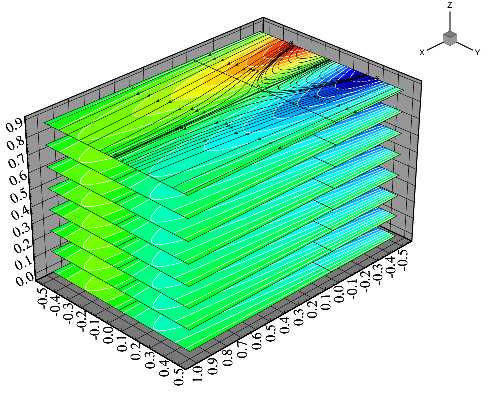
\includegraphics[width=0.65\textwidth]{kovas3_bitmap.eps}
\end{center}
\caption{
\label{kov3soln}
  Solution to the \texttt{kovas3} problem, visualized using
  \emph{Tecplot}.  The plot shows contours of $v$ velocity component
  and streamlines.  }
\end{figure}

%============================================================================
\section{Vortex breakdown\,---\,a cylindrical-coordinate problem}
\label{sec.vb}

Here we will examine a problem which uses the cylindrical coordinate
option of \verb+dns+.  The physical situation is a cylindrical cavity,
$H/R=2.5$ with the flow driven by a spinning lid at one end.  At the
Reynolds number we'll use, $\Rey=\Omega R^2/\nu=2119$, a vortex
breakdown is known to occur.  The flow in this case is invariant in
the azimuthal direction, but has three velocity components (it is
2D/3C).  In the cylindrical code, the order of spatial directions and
velocity components is $z$, $r$, $\theta$.

Note that for a full circle in the azimuthal direction, \texttt{BETA =
  1.0}, (which is the default value). In fact, the value would not be
used in the present solution, since all derivatives in the azimuthal
direction are implicitly zero when \verb+N_Z=1+. (But see
\S\,\ref{sec.cbcs} below.)

{\small
\begin{verbatim}
#############################################################################
# 15 element driven cavity flow.

<FIELDS>
        u v w p
</FIELDS>

<TOKENS>
        CYLINDRICAL = 1
        N_Z         = 1
        BETA        = 1.0
        N_TIME      = 2
        N_P         = 11
        N_STEP      = 100000
        D_T         = 0.01
	Re          = 2119
        KINVIS      = 1/Re
        OMEGA       = 1.0
        TOL_REL     = 1e-12
</TOKENS>

<GROUPS NUMBER=3>
        1       v       velocity
        2       w       wall
        3       a       axis
</GROUPS>

<BCS NUMBER=3>
        1       v       4
                        <D>     u = 0           </D>
                        <D>     v = 0           </D>
                        <D>     w = OMEGA*y     </D>
                        <H>     p               </H>
        2       w       4
                        <D>     u = 0           </D>
                        <D>     v = 0           </D>
                        <D>     w = 0           </D>
                        <H>     p               </H>
        3       a       4
                        <A>     u               </A>
                        <A>     v               </A>
                        <A>     w               </A>
                        <A>     p               </A>
</BCS>

<NODES NUMBER=24>
        1       0       0       0
        2       0.4     0       0
        3       0.8     0       0
        4       1.5     0       0
        5       2.4     0       0
        6       2.5     0       0
        7       0       0.15    0
        8       0.4     0.15    0
        9       0.8     0.15    0
        10      1.5     0.15    0
        11      2.4     0.15    0
        12      2.5     0.15    0
        13      0       0.75    0
        14      0.4     0.75    0
        15      0.8     0.75    0
        16      1.5     0.818   0
        17      2.4     0.9     0
        18      2.5     0.9     0
        19      0       1       0
        20      0.4     1       0
        21      0.8     1       0
        22      1.5     1       0
        23      2.4     1       0
        24      2.5     1       0
</NODES>

<ELEMENTS NUMBER=15>
        1       <Q>      1  2  8  7     </Q>
        2       <Q>      2  3  9  8     </Q>
        3       <Q>      3  4 10  9     </Q>
        4       <Q>      4  5 11 10     </Q>
        5       <Q>      5  6 12 11     </Q>
        6       <Q>      7  8 14 13     </Q>
        7       <Q>      8  9 15 14     </Q>
        8       <Q>      9 10 16 15     </Q>
        9       <Q>     10 11 17 16     </Q>
        10      <Q>     11 12 18 17     </Q>
        11      <Q>     13 14 20 19     </Q>
        12      <Q>     14 15 21 20     </Q>
        13      <Q>     15 16 22 21     </Q>
        14      <Q>     16 17 23 22     </Q>
        15      <Q>     17 18 24 23     </Q>
</ELEMENTS>

<SURFACES NUMBER=16>
        1       1       1       <B>     a       </B>
        2       2       1       <B>     a       </B>
        3       3       1       <B>     a       </B>
        4       4       1       <B>     a       </B>
        5       5       1       <B>     a       </B>
        6       5       2       <B>     v       </B>
        7       10      2       <B>     v       </B>
        8       15      2       <B>     v       </B>
        9       15      3       <B>     w       </B>
        10      14      3       <B>     w       </B>
        11      13      3       <B>     w       </B>
        12      12      3       <B>     w       </B>
        13      11      3       <B>     w       </B>
        14      11      4       <B>     w       </B>
        15      6       4       <B>     w       </B>
        16      1       4       <B>     w       </B>
</SURFACES>
\end{verbatim}
}

The mesh for the problem is shown in figure~\ref{vb1msh}, and the
velocity field is shown compared to an experimental streakline flow
visualisation on the front cover of this document.
\begin{figure}
\begin{center}
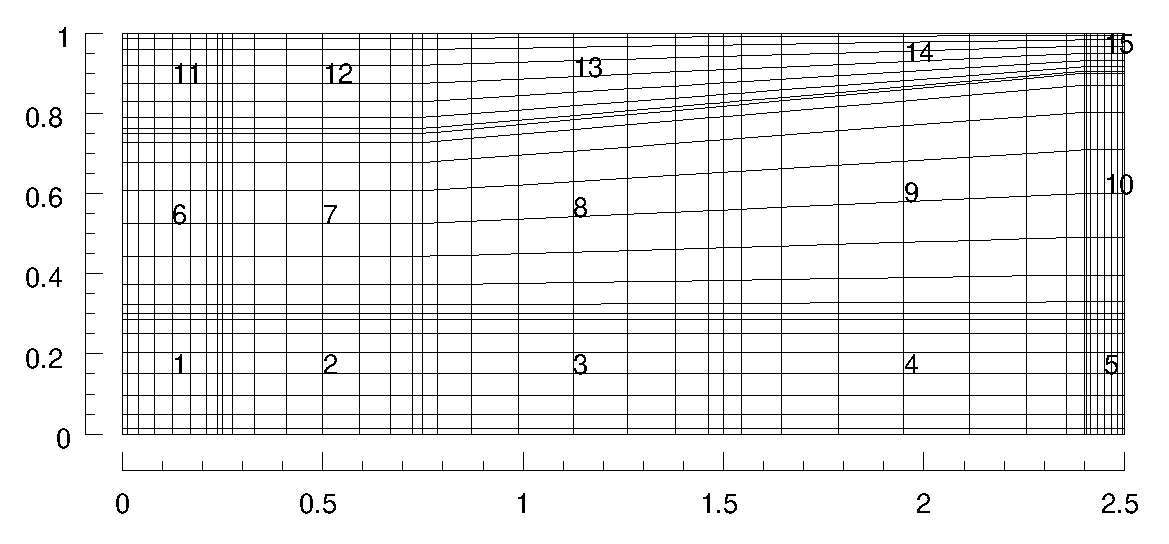
\includegraphics[width=0.6\textwidth]{vb1mesh.eps}
\end{center}
\caption{
\label{vb1msh}
  Mesh for the vortex breakdown problem.  The spinning lid is at right.
  }
\end{figure}

%----------------------------------------------------------------------------
\subsection{BCs for cylindrical coordinates}
\label{sec.cbcs}

A new feature here is the use of BCs of type \verb+A+ on the axis of
the flow.  Internally, the code sets the BC there either as zero
essential or zero natural, depending on the physical variable and the
Fourier mode.  Owing to the coupling scheme used in the code
\citep{blsh04}, the boundary conditions for the radial and azimuthal
velocities \verb+v+ and \verb+w+ must be of the same type within each
group.  A further restriction is that the group to which the axis
belongs must have name \verb+axis+.

Finally, say you wish to solve a cylindrical-coordinate problem where
you know there is an $n$-fold azimuthal symmetry (say $n=3$). In that
case, it is much cheaper to solve with \verb+BETA=3+, and use
one-third the number of azimuthal planes that would be required for
\verb+BETA=1+.

%=============================================================================
\section{Boundary condition roundup}
\label{sec.bcs}

The basic types of boundary conditions the code can deal with are
Dirichlet type (value of variable is set, a.k.a.\ an \emph{essential}
boundary condition in the finite element community) and Neumann type
(boundary-normal gradient of value is approximated, a.k.a.\ a
\emph{natural} type boundary condition in the finite-element
community). The code can also deal with boundary conditions of mixed
type (a linear combination of Dirichlet and Neumann). We note that
periodic domain boundary surfaces (\verb|<P>|) are allowed, but
strictly speaking, periodicity does not constitute a boundary
condition as such.  Also we remark that for our code(s), boundary
conditions may only be set for variables involved in elliptic
sub-problems where, owing to the MWR treatment, Neumann boundary
conditions are implemented as integral approximations (which converge
to the given value pointwise as resolution is increased), while
Dirichlet conditions are `lifted' out of the problem and imposed
exactly to the values which are set by the user.

Standard Dirichlet and Neumann boundary conditions may be supplied as
a string that can be parsed by the solver to obtain a real value,
based on predefined and user-declared \verb|TOKENS|, and also the
space/time variables \verb|x|, \verb|y|, \verb|z| and \verb|t|.  These
strings are re-parsed at each time step, so time-varying boundary
conditions are allowed. We have already seen examples of these BC
declarations in \S\S\,\ref{sec.laplace}, \ref{sec.kovas}
and~\ref{sec.vb}.  Note that the strings involved should not contain
white space.  

We have not yet described mixed boundary conditions.  These are of
type $\partial c/\partial n+K(c-C)=0$ where $C$ and $K$ are constants.
Here, $n$ signifies the unit outward normal direction: $\partial
c/\partial n=\bm{n\cdot\nabla c}$.  Mixed boundary conditions are
specified in the form \verb|<M> field = mulval;refval </M>| where
\verb|mulval| is (a string that evaluates to) the real value $K$ and
\verb+refval+ is (a string that evaluates to) the real value $C$.  At
present for mixed BCs, unlike Dirichlet and Neumann boundary
conditions, $C$ and $K$ are fixed at the values they initially
evaluate to (not time-varying).

In \NavSto\ type problems, various of the above boundary conditions
for the velocity and pressure variables are typically combined in set
ways.  In some cases, the user does not provide values or choose the
combination since the boundary conditions are computed internally.
Below we supply as examples various typical boundary condition sets
which would be located in the \verb+BCS+ section of a session file.
As written, they are for \twoc\ \NavSto\ problems but the
generalisation to \threec\ problems should be obvious.

See also \S\,3.2 of the \Dog\ user guide for a discussion of sets of
boundary condtions appropriate for symmetry and anti-symmetry
boundaries.

%-----------------------------------------------------------------------------
\subsection{No-slip wall}

{\small
\begin{verbatim}
  <D> u = 0.0 </D>
  <D> v = 0.0 </D>
  <H> p       </H>
\end{verbatim}
}
\noindent The tag \verb+H+ for pressure (\verb+p+) denotes an
internally computed 'high-order' Neumann condition, as originally
described by \citet{kio91}.  If the associated \verb|GROUP| string is
\verb|wall| then tractions will contribute to the integrated values
found in \verb+session.flx+ file, see \S\,\ref{sec.flux}.

%-----------------------------------------------------------------------------
\subsection{Inflow or prescribed-velocity boundary}

{\small
\begin{verbatim}
  <D> u = 1.0 </D>
  <D> v = 0.0 </D>
  <H> p       </H>
\end{verbatim}
}
\noindent Note that either of the supplied values can be a string to
be evaluated by the parser at each timestep.

%-----------------------------------------------------------------------------
\subsection{Slip (no-penetration) boundary}

{\small
\begin{verbatim}
  <N> u = 0.0 </N>
  <D> v = 0.0 </D>
  <H> p       </H>
\end{verbatim}
}
\noindent Note that in this case, the boundary needs to be aligned
with the $x$ axis.  At present there is no way to set a slip boundary
which is inclined or curved; it must be parallel to either the $x$ or
$y$ axis.

%-----------------------------------------------------------------------------
\subsection{`Stress-free' outflow boundary}
\label{sec.stressfree}

{\small
\begin{verbatim}
  <N> u = 0.0 </N>
  <N> v = 0.0 </N>
  <D> p = 0.0 </D>
\end{verbatim}
}
\noindent This is a restricted approximation to a true stress-free
boundary where the tractions are zero. This boundary is also
stress-free but achieves the condition by ensuring that the viscous
and pressure tractions are individually zero, rather than their sum.

%-----------------------------------------------------------------------------
\subsection{`Robust' outflow boundary}
\label{sec.robust}

{\small
\begin{verbatim}
  <O> u </O>
  <O> v </O>
  <O> p </O>
\end{verbatim}
}
\noindent This is a set of computed boundary conditions (computed
Neumann for velocity and computed Dirichlet for pressure).  (In fact
if \verb+w+ is included, its boundary condition is set as $\partial
w/\partial n=0$ rather than being computed.) This boundary condition
was originally described in \citet{dkc14}, and is based on maintaining
boundedness of kinetic energy within the domain.  It is excellent for
maintaining stability for flows in short open domains, where the use
of the 'stress-free' condition described in \S\,\ref{sec.stressfree}
can lead to catastrophe if significant inflow occurs over an outflow
boundary.  Type \verb|O| boundaries must set the string \verb|outflow|
in their associated \verb|GROUP|.

%-----------------------------------------------------------------------------
\subsection{Axis boundary}

{\small
\begin{verbatim}
  <A> u </A>
  <A> v </A>
  <A> p </A>
\end{verbatim}
}
\noindent
This is a set of Fourier-mode dependent homogeneous Dirichlet and
Neumann boundary conditions to be used when the boundary coincides
with the $x$ axis of a cylindrical coordinate system as described in
\citet{blsh04}. Type \verb|A| boundaries must set the string
\verb|axis| in their associated \verb|GROUP|.

%=============================================================================
\section{Fixing problems}
\label{sec.fix}

You are liable to come up against a few generic problems when making
and running your own cases. Here we will restrict discussion to
\NavSto\ problems and \verb+dns+. The best diagnostic of trouble is
the divergence of the solution. The code will output an estimate of
the CFL-timestep every \verb+IO_CFL+ timesteps (default 50), along
with the average divergence of the solution (in the operator-splitting
used, incompressibility is only ensured in the spatial-convergence
limit). Unfortunately the CFL estimate is presently unreliable, but
the divergence energy provides an excellent diagnostic of trouble!  If
velocity and length scales are of order unity, the reported divergence
energy should be much less than unity; if the divergence is large then
either the solution is blowing up\footnote{One wag suggested the name
  \Semtex\ was associated with this property of the solutions.}, or
the spatial resolution is inadequate, or both.

By far the most common problem is that the solution will have a
CFL-type instability brought about by using too large a time-step;
this instability is unavoidably associated with using explicit time
integration for the advection terms in the \NavSto\ equations. This
problem is easily enough fixed: try reducing \verb+D_T+ and increasing
\verb+N_STEP+ to maintain the same integration interval. Obviously you
will typically want \verb+D_T+ as large as possible, so if the problem
runs stably, increase the timestep as much as is reasonable. If the
velocity and timescales are of order unity, then the maximum timestep
would typically be of order two orders of magnitude smaller
(\verb+0.01+). Note that CFL-stability will decrease with increasing
time-integration order (\verb+N_TIME+).

If the solution persists in blowing up when the timestep is reduced,
the next most common cause is that there is inflow across an outflow
boundary (in which case the problem is ill-posed, however, in practice
\emph{some} inflow across an outflow boundary over restricted times
may be present without causing difficulty). To check if this is the
cause, you could put some history points near the outflow (see
\S\,\ref{sec.history}), but the best method of diagnosis is to run the
solution up to a time when divergence starts to increase markedly,
then use \emph{Tecplot} or some other postprocessor to examine the
solution near the outflow.  This problem has been largely circumvented
in \Semtex~V8 using the robust outflow BC set described by
\citet{dkc14}, see \S\,\ref{sec.robust} above, though it cannot
overcome all problems (\eg an `outflow' boundary with completely
dominant inflow).  In pathological cases of this sort, fixing the
problem will generally require the mesh to be altered: sometimes the
mesh is badly structured near the outflow (\eg element sizes have been
varied too rapidly); sometimes the problem can be overcome by
extending the domain downstream; sometimes the domain needs to be
reshaped (\eg by contracting it in the cross-flow direction) so that
there will be no outflow over the inflow boundary. If all else fails,
consider the methods of \S\,\ref{sec.sponge} to force the velocity
near the outflow to be something more computationally tractable (if
unphysical).

Any time you change the element polynomial order by changing
\verb+N_P+, or alter the structure of the boundary conditions, you
should remake the numbering file \verb+session.num+. It is especially
important to remember this if you have changed the structure of the
boundary conditions without changing element order, as no warning will
be triggered; however, in this case you may no longer be actually
applying the boundary conditions you have set in the session file
because the \verb+mask+ values in \texttt{session.num} (which are set
to \verb+1+ along a Dirichlet-type boundary) may no longer match what
is implied by \texttt{session}.

%=============================================================================
\section{Execution speed}
\label{sec.speed}

\Semtex\ relies heavily on the BLAS, so it can be worth seeking fast
implementations. Especially, performance of matrix--matrix
multiplication routine \verb+dgemm+ is critical. Consistently of late,
Kazushige Goto's implementation of the BLAS gives best performance and
is worth seeking out, although I understand his \verb+dgemm+ has also
now been licenced to various vendors (Intel, AMD, Apple, \ldots) and
is what you'll get if you link their extended math libraries.

As Reynolds numbers increase (\ie \verb+KINVIS+ decreases), the
viscous Helmholtz matrices in the operator splitting become more
diagonally dominant and better conditioned. In this case, you may find
that iterative (PCG) solution of the viscous step (obtained by setting
\verb|ITERATIVE=1| or running \verb|dns -i|) is actually faster than
the direct solution that is obtained by default. This is nice because
additionally, less memory is required. It is generally worth checking
this if you plan an extended series of runs, and Reynolds numbers are
large.

%%%%%%%%%%%%%%%%%%%%%%%%%%%%%%%%%%%%%%%%%%%%%%%%%%%%%%%%%%%%%%%%%%%%%%%%%%%%%%
\chapter{Extra controls}

This chapter describes some additional features that are implemented
within the \NavSto\ solver \verb+dns+ to control execution and
output.

%=============================================================================
\section{Default values of flags and internal variables}
\label{sec.default}

There are two simple ways to establish the default values of all the
internal flags and variables used by \Semtex. The first is via
the \verb+calc+ utility: run \verb+calc -h+ and check the output (this
will also show you all the functions available to the parser for
calculating \verb+TOKEN+ variables, initial and boundary
conditions). The second is to examine the file
\verb+femlib/defaults.h+.

%=============================================================================
\section{Checkpointing}
\label{sec.check}

By default, intermediate solutions are written out as checkpoint dumps
in file \verb+session.chk+ every \verb+IO_FLD+ steps (default value
\verb+IO_FLD = 500+), rotating this to \verb+session.chk.bak+ so there
are usually two checkpoint files available for restarting if execution
stops prematurely (\eg if terminated by a queuing system or by a
floating point error).  Once the final time (\verb+N_STEP+) is
reached, the outcome (the termimal solution field) is written to
\verb+session.fld+.

Sometimes however, one wants a sequence of field dumps to be written
to \verb+session.fld+.  One can toggle this behaviour on the command
line using \verb+dns -chk+, or alternatively set the \verb+TOKEN+
\verb+CHKPOINT=0+ (the default being \verb+CHKPOINT=1+).  Note that
turning off checkpointing can result in the generation of extremely
large \verb+session.fld+ files.

%=============================================================================
\section{Iterative solution}
\label{sec.iterative}

Two matrix solution methods are implemented for Helmholtz problems
associated with the viscous substep of the time splitting.  By
default, direct Schur-complement solutions are used.  The associated
global matrices can consume quite large amounts of memory, typically
much more than is required for storage of the associated field
variable.  Iterative (PCG) solution can also be selected, and this has
the advantage that since it is matrix-free, no global matrices are
required, however, solution may be slower than for the direct solver
(depending on the condition number of the global matrix problem).

The token that controls the selection of matrix solution method is
\verb+ITERATIVE+.  For \verb+dns+, PCG solution can be selected for
the viscous substep of the solution (\verb+ITERATIVE = 1+).  This can
also be selected via a command-line option (\verb+dns -i+), but note
that this overridden by tokens set in the \verb+session+ file (the
default value is \verb+ITERATIVE = 0+).

Iterative solution can be useful for the viscous substep, particularly
when the Reynolds number is high, since this decreases the condition
number of the associated global matrices.  In fact, iterative
solutions for the viscous substep can execute faster than direct
solutions at high Reynolds number, although this is platform
dependent. You should always consider trying \verb+ITERATIVE = 1+ as
an option for simulations where the Reynolds number is more than a few
hundred.

%=============================================================================
\section{Wall fluxes}
\label{sec.flux}

A file called \verb+session.flx+ is used to store the integral over
the \verb+wall+ group boundaries of viscous and pressure stresses
(i.e.\ lift and drag forces).  Output is done every \verb+IO_HIS+
steps.  For each direction ($x$, $y$, $z$), the outputs are in turn
the pressure, viscous, and total force per unit length.  In 2D the
$z$-components are always zero, while in 3D the $z$-component pressure
force is always zero, owing to the fact that the geometry is invariant
in that direction.  For cylindrical geometries, the output values are
forces per radian (in the $x$ and $y$ directions) and torque per
radian (in the $z$ direction) rather than forces per unit length.

%=============================================================================
\section{Wall tractions}
\label{sec.traction}

If the token \verb+IO_WSS+ is set to a non-zero value then the normal
and the single (2D) or two (3D) components of tangential boundary
traction are computed on the \verb+wall+ group, and output every
\verb+IO_WSS+ steps in the file \verb+session.wss+.  This is a binary
file with structure similar to a field dump.  The utility
\verb+wallmesh+ is used to extract the corresponding mesh points
along the walls.

%=============================================================================
\section{Modal energies}
\label{sec.modal}

For \threed\ simulations (\verb+N_Z > 2+), a file of modal energies,
\verb+session.mdl+, is produced.  This provides valuable diagnostic
information for turbulent flow simulations.  For each active Fourier
mode $k$ in the simulation, the value output every \verb+IO_HIS+ steps
is 
\[
E_k =
\frac{1}{2A}\int_\Omega
\hat{\bm{u}}_k^\ast\cdot\hat{\bm{u}}_k \,{\rm d}\Omega,
\]
where $A$ is the area of the 2D domain~$\Omega$.  (In cylindrical
coordinate problems, the integrand is multiplied by radius.) Each line
of the file contains the time $t$, mode number $k$ and $E_k$.

We note that the energies are output only for non-negative Fourier
modes.  To get the correct estimates for the one-sided spectrum (and
to satisfy Parseval's relation), the energies for non-zero modes
should be doubled.

%=============================================================================
\section{History points}
\label{sec.history}

History points are used to record solution variables at fixed spatial
locations as the simulation proceeds.  The locations need not
correspond to grid points, as data are interpolated onto the given
spatial locations using the elemental basis functions.  Locations of
history points are declared in the \verb+session+ file as follows:
\begin{verbatim}
<HISTORY NUMBER=1>
#       tag     x       y       z 
        1       0       0       0
</HISTORY>
\end{verbatim}

A file called \verb+session.his+ is produced as output.  Each line of
the file contains the step number, the time, the history point tag
number, followed by values for each of the solution variables.  The
step interval at which history point information is dumped to file is
controlled by the \verb+IO_HIS+ token; the default value is
\verb+IO_HIS = 10+.

%=============================================================================
\section{Averaging}
\label{sec.average}

Set \verb+AVERAGE = 1+ in the tokens section to get averages of field
variables left in files \verb+session.ave+ and \verb+session.avg+
(which are analogous to \verb+session.chk+ and \verb+session.fld+, but
\verb+session.ave.bak+ is not produced).  Averages are updated
every \verb+IO_HIS+ steps, and dumped every \verb+IO_FLD+ steps.
Restarts are made by reading \verb+session.avg+ if it exists.

Setting \verb+AVERAGE = 2+ will accumulate averages for Reynolds
stresses as well, with reserved names \verb+ABCDEF+, corresponding to
products
\begin{verbatim}
uu uv uw     A  B  D
   vv vw  =     C  E
      ww           F
\end{verbatim}
The hierarchy is named this way to allow accumulation of products in 2D
as well as 3D (for 2D you get only \verb+ABC+).  In order to actually
compute the Reynolds stresses from the accumulated products you need
to run the \verb+rstress+ utility, which subtracts the products of the
means from the means of the products:
\begin{verbatim}
rstress session.avg > reynolds-stress.fld
\end{verbatim}
An alternative function of \verb+rstress+ is to subtract one field
file from another:
\begin{verbatim}
rstress good.fld test.fld | convert | diff
\end{verbatim}

Setting \verb+AVERAGE = 3+ will accumulate sums of additional products
for computation of terms in the energy transport equation. You will
then need to use the \verb+eneq+ utility to actually compute the
terms. Presently this part of the code is only written for Cartesian
coordinates.

%=============================================================================
\section{Phase averaging}
\label{sec.phase}

Phase averaging is useful for turbulent flows with a dominant (and
known) underlying temporal period.  We can collect statistics (with
\verb|AVERAGE=1|, \verb|2| or \verb|3|)\,---\,much as for the case
without phase averaging enabled\,---\,conditional on phase in the
cycle of the underlying period, see \citet{rehu72}.  Turning
on phase averaging does not preclude or stop collection of standard
statistics.  The enabling token is \verb|N_PHASE|, which must be a
positive integer; in addition one needs token \verb|STEPS_P| (steps
per period) which must be chosen such that \verb|STEPS_P| modulo
\verb|N_PHASE| is zero, and also \verb|N_STEP| modulo \verb|N_PHASE|
must be zero \emph{and} \verb|IO_FLD=STEPS_P/N_PHASE|.  Statistics are
written to files \verb|session.0.phs| \ldots \verb|session.X.phs|
where \verb|X=N_PHASE-1|.  The Reynolds stresses computed from these
files will represent fluctuations around the conditional average flow
at each phase point (the so-called `triple decomposition').

The slight difficulty is that if the period is not very well-defined
or we have a poor estimate of it, our sampling phase will slowly drift
unless we take corrective action.  However if the underlying period is
very well defined (\eg the flow is periodically forced) the method has
great potential.

%=============================================================================
\section{Particle tracking}
\label{sec.particle}

The code allows for tracking of massless particles, but this only
works correctly for non-concurrent execution at present.  Tracking is
quite an expensive operation, since Newton--Raphson iteration is used
to relocate particles within each element at every timestep.

The application looks for a file called \verb+session.par+.  Each line
of this file is of form
\begin{verbatim}
#     tag  time  ctime  x     y      z
      1    0.0   0.0    1.0   10.0   0.5.
\end{verbatim}
The \verb+time+ value is the integration time, while \verb+ctime+
records the time at which integration was initialised.

Output is of the same form, and is called \verb+session.trk+.  The use
of separate files, rather than by declaration in the session file, is
intended so that \verb+session.trk+ files can be moved to
\verb+session.par+ files for restarting.  Particles that aren't in the
domain at startup, or leave the domain during execution, are deleted.

Setting \verb+SPAWN = 1+, re-initiates extra particles at the original
positions every timestep.  With spawning, particle tracking can
quickly grow to become the most time-consuming part of execution.

%=============================================================================
\section{Spectral vanishing viscosity}
\label{sec.svv}

Spectral vanishing viscosity (SVV) amounts to implementing larger
viscosity at higher wavenumbers either in Fourier space or in spectral
element polynomial space.  The idea is that as resolution is increased
via $p$-refinement, the effect `vanishes' \citep{tadmor89,mot93}.  One
may regard SVV either as a type of implicit large-eddy simulation
methodology \citep{pasquetti06} or as a means of stabilizing spectral
element solutions especially at high Reynolds numbers
\citep{xupa04,kish06}. Neither of these ideas has firm theoretical
underpinning at this stage, yet the method does appear quite effective
in reducing resolution requirements for turbulent flow simulations
\citep{ksb12,cnbmo15}.  Our implementation and nomenclature follows
the `standard method' described in \citet{ksb12}.  One can turn on SVV
separately and with different parameters for ($x$,\,$y$) spectral
elements and in the Fourier ($z$) direction.  These are all declared
in the \verb+TOKENS+ section.

\begin{tabbing}
XXXXXXX \= \kill
\texttt{SVV\_MN} \> Corresponds to cut-in mode $M_{zr}$ in 
spectral elements. Must be less than \texttt{N\_P}.\\ 
%
\texttt{SVV\_MZ} \> Corresponds to cut-in mode $M_\varphi$ in 
Fourier direction. Must be less than \texttt{N\_Z/2}.\\
%
\texttt{SVV\_EPSN} \> Corresponds to $\varepsilon_{zr}$. 
Should be a value larger than \texttt{KINVIS}, \eg \texttt{5*KINVIS}.\\
%
\texttt{SVV\_EPSZ} \> Corresponds to $\varepsilon_\varphi$. 
A value larger than \texttt{KINVIS}.
\end{tabbing}

The default polynomial transform in to place spectral element
expansions into a discrete hierarchical space is the discrete Legendre
transform \citep[see e.g.][]{blsc03}. This can be changed in
\verb|src/svv.cpp|.

%=============================================================================
\section{General body forcing}
\label{sec.dns_ff}

\textsl{This extension was developed by Thomas Albrecht.}\\

\noindent
If found, the \verb+FORCE+ section of the session file allows you to
declare various types of body forcing, \ie add a source term
to the RHS of the \NavSto\ equation. The currently implemented types
include (any combination allowed):\\[1em]
\begin{tabular}{rll}
 $ \bm{f} =$ & $\bm{f}_{const}$                           
  & constant force \\
           $+$ & $\bm{a_1}(\bm{x})$                       
  & steady, but spatially varying force\\
           $+$ & $\bm{a_2}(\bm{x}) \, \bm{\alpha}(t) $ 
  & modulated force\\
           $-$ & $m_1(\bm{x})\,(\bm{u} - \bm{u}_0)$  
  &  sponge region\\
           $-$ & $m_2(\bm{x})\,(\bm{u}/|\bm{u}|)\,|\bm{u}(\bm{x}, t)|^2$  
  &  `drag' force  \\
%            + & $\bm{d} \, c$                         &  bouyancy \\
           $+$ & $\bm{\epsilon} G$                        
  &  white noise    \\
           $-$ & 2 $\bm{\Omega} \times \bm{u} - 
                    (\cd\bm{\Omega}/\cd t) \times \bm{x} -
                    \bm{\Omega} \times \bm{\Omega} \times \bm{x}$  
  &  Coriolis force. \\
\end{tabular}\\[1em]
%----------------------------------------------------------------------------
% \subsection{Constant force}

\noindent For example, a force constant in time and space $\bm{f} =
\bm{f}_{const}$ is declared by:
\begin{verbatim}
<FORCE>
        CONST_X = 4
        CONST_Y = 0
        CONST_Z = 0
</FORCE>
\end{verbatim}
This type of forcing must not be time or space dependent. It is suitable
for periodic channel flow, where you have a uniform and steady force
driving the flow, see \verb+channel-FX+ for an example session.

Except for the constant force, all forcing terms are applied in
physical space.

Unless otherwise noted, any skipped keyword defaults to 0. Any line
starting with a hash \verb+#+ is ignored.

%----------------------------------------------------------------------------
\subsection{Steady force}

A spatially varying, steady force $\bm{f} = \bm{a}(\bm{x})$, computed
(or read from a file) during pre-processing and applied every time
step. See \verb|box-steady| for the complete example session. It suits
applications requiring localised, steady forcing.
\begin{verbatim}
<FORCE>
        STEADY_X =  cos(x)
        STEADY_Y = -sin(z)
        STEADY_Z = -cos(y)
        # STEADY_FILE = box-steady.force.fld
</FORCE>
\end{verbatim}

You may also point \verb+STEADY_FILE+ to a field file, in which case
the force is taken from the \verb+uvw+ fields of that file and
\verb+STEADY_[XZY]+ is ignored.
% The steady force may also be read from a field file by pointing
% \verb+STEADY_FILE = +$<$\textit{aFileName}$>$ to it. If so, the
% \verb+STEADY_[XZY] =+ lines are ignored, and the force is taken from
% \verb+lmn+ fields of the given file.\\[1em]
% \noindent\verb+compare box-steady > box-steady.force.fld+\\
% \verb+head box-steady.force.fld | grep Fields+\\
% \verb+uvwp+\fbox{\texttt{lmn}}\verb+                   Fields written+

%----------------------------------------------------------------------------
\subsection{Modulated force}

A spatially varying force, which is modulated in time, $\bm{f} =
\bm{a}(\bm{x}) \, \bm{\alpha(t)} $. The steady part $\bm{a}(\bm{x})$ is
computed (or read from a file) during pre-processing, while
$\bm{\alpha(t)}$ is evaluated each time step. See \verb|box-mod| for
the complete example session.
\begin{verbatim}
<FORCE>
        # -- spatially varying part
        MOD_A_X =  cos(x)
        MOD_A_Y = -sin(z)
        MOD_A_Z = -cos(y)
        # MOD_A_FILE = box-mod.force.fld

        # -- time varying part
        MOD_ALPHA_X = step(t, 10)
        MOD_ALPHA_Y = step(t, 10)
        MOD_ALPHA_Z = step(t, 10)
</FORCE>
\end{verbatim}

%----------------------------------------------------------------------------
\subsection{Sponge region}
\label{sec.sponge}

This implements a so-called `sponge region' defined by the shape
function $m(x)$ in which a (physically meaningless) penalty term
$\bm{f} = m(\bm{x}) \, (\bm{u} - \bm{u}_0)$ forces the flow towards a
given solution $\bm{u}_0$.  It is especially useful for
inflow--outflow simulations of vortex shedding or turbulence: if the
velocity fluctuations hit the outflow boundary condition, they cause
unphysical reflections back into the domain which distort the upstream
flow. A sponge region placed just upstream the outflow boundary helps
to reduce the velocity fluctuations to (near) zero and thereby prevents
those reflections. The following section would apply the penalty term
for $20 \le x \le 24$, and within that region forces the velocity to
approach~$(1, 0, 0).$ That given solution may be a function of space,
but must be steady.
\begin{verbatim}
<FORCE>
        SPONGE_M = 5. * step(x,20)*heav(24-x)
        SPONGE_U = 1
        SPONGE_V = 0
        SPONGE_W = 0
</FORCE>
\end{verbatim}
See \verb|cylinder17-sponge| for a more advanced example session.

%----------------------------------------------------------------------------
\subsection{'Drag' force}

An approximate drag force
$\bm{f} = - m(\bm{x}) \, (\bm{u}/|\bm{u}|)\, |\bm{u}(\bm{x},
t)|^2$.
Be aware that we use the previous time step's velocity $\bm{u}^{n}$ here.
\begin{verbatim}
<FORCE>
        DRAG_M = heav((x-2)^2 + y^2, 0.25)
</FORCE>
\end{verbatim}
See \verb+channel-FX-drag+ for an example session, where the drag
force is applied in a circular region centered around (2, 0.5) in a
laminar channel flow.

%----------------------------------------------------------------------------
\subsection{White noise force}

Similar to the \verb+noiz+ tool, this continuously adds random
perturbation $\bm{f} = (\epsilon_x, \epsilon_y, \epsilon_z)^T\,G$ in
specified direction, where $G$ is a normal distributed random
variable. Setting $\verb+WHITE_MODE+ \ge 0$ perturbs the given mode
only, \ie \verb+WHITE_MODE = 2+ will perturb mode 2 only. Omitting
this keyword or setting $\verb+WHITE_MODE+ < 0$ will apply white noise
to all modes.

The following example applies white noise in $x-$direction to mode 0:
\begin{verbatim}
<FORCE>
        WHITE_MODE = 0
        WHITE_EPS_X = 0.1
        WHITE_EPS_Y = 0
        WHITE_EPS_Z = 0
</FORCE>
\end{verbatim}
Adding white noise in all three directions degrades performance by
about 10\%. See \verb+channel-FX-noiz+ for an example session.

%----------------------------------------------------------------------------
\subsection{Rotating frame of reference: Coriolis and centrifugal force}

See \citet{ablmm15} for an example of DNS carried out in a rotating
frame of reference.

% @book{batchelor2000,
%   title={An introduction to fluid dynamics},
%   author={Batchelor, G.K.},
%   year={1967},
%   publisher={Cambridge University Press}
% }

If the flow is to be computed in a rotating frame of reference,
additional acceleration terms appear, namely $\bm{f} = -2\,\bm{\Omega}
\times \bm{u} - (\cd\bm{\Omega}/\cd t) \times \bm{x} -\bm{\Omega}
\times (\bm{\Omega} \times \bm{x})$ \citep{bat67}. The vector
of rotation $\bm{\Omega}$ is \emph{always} given in Cartesian
co-ordinates, even if \verb|CYLINDRICAL = 1|. Its magnitude and/or
orientation can change with time. However, the axis of rotation it is
always assumed to go through the origin. Depending on whether
$\bm{\Omega}$ is steady or not, usage slightly differs.


For unsteady $\bm{\Omega}$, set the flag \verb|CORIOLIS_UNSTEADY = 1|
and give $\bm{\Omega}$ and $\cd\bm{\Omega}/\d t$. All terms are
re-evaluated each time step.
\begin{verbatim}
<TOKENS>
        f        = 1.
        omega    = TWOPI * f
</TOKENS>

<FORCE>
        CORIOLIS_UNSTEADY = 1

        CORIOLIS_OMEGA_X = 0
        CORIOLIS_OMEGA_Y = 0
        CORIOLIS_OMEGA_Z = omega * sin(t)

        CORIOLIS_DOMEGA_X_DT = 0
        CORIOLIS_DOMEGA_Y_DT = 0
        CORIOLIS_DOMEGA_Z_DT = omega * cos(t)
</FORCE>
\end{verbatim}

\noindent 
For constant $\bm{\Omega}\neq f(t)$, the term
$-(\cd\bm{\Omega}/\cd t)\times\bm{x}$ vanishes, and the centrifugal
force $-\bm{\Omega} \times (\bm{\Omega} \times \bm{x})$ can be
computed during pre-processing.
%
Set \verb|CORIOLIS_UNSTEADY = 0| and make sure to include the centrifugal
force manually using a steady force as it is no longer computed automatically%
\footnote{If you're lazy, or for cross-checking, you could set
  \texttt{CORIOLIS\_UNSTEADY = 1} and omit
  \texttt{CORIOLIS\_DOMEGA\_[XYZ]\_DT} to have the centrifugal term
  computed automatically. Note, however, that this degrades
  performance as it is done each time step.}.  A temporal derivative
$\cd\bm{\Omega}/\cd t$, if given, is ignored.

\begin{verbatim}
<FORCE>
        CORIOLIS_UNSTEADY = 0

        CORIOLIS_OMEGA_X = 0
        CORIOLIS_OMEGA_Y = 0
        CORIOLIS_OMEGA_Z = omega

        # -- centrifugal term for Omega = (0, 0, omega)^T
        #    for a cylindrical problem
        STEADY_X = x*omega^2
        STEADY_Y = omega^2*y*(cos(z)^2)
        STEADY_Z = -omega^2*y*cos(z)*sin(z)
</FORCE>
\end{verbatim}

% A sample session \verb+box-coriolis+ makes use of steady forcing to let
% the flow approach a given (divergence-free) solution, taking into
% account this coriolis term.
%\noindent See \verb|cylkovrot| for an example session.

%%%%%%%%%%%%%%%%%%%%%%%%%%%%%%%%%%%%%%%%%%%%%%%%%%%%%%%%%%%%%%%%%%%%%%%%%%%%%%
\chapter{Specialised executables}

The special compilations below can be combined.

%=============================================================================
\section{Concurrent execution}
\label{sec.parallel}

The code supports concurrent execution for 3D simulations, with MPI
used as the message-passing kernel. Compile using \verb+make MPI=1+ to
produce \verb+dns_mp+. (You will also need to compile in the
appropriate message-passing routines in compiling \verb+femlib+, for
which change to the \verb+femlib+ directory, then do
\verb+make clean; make MPI=1; make install MPI=1+.)  Nonlinear terms
are not dealiased when running in parallel, but are dealiased in the
Fourier direction when running on one process, or running the serial
code. To get a serial code that does not perform dealiasing on Fourier
terms (e.g.\ for cross-checking), compile the serial code using
\verb+make ALIAS=1+ to produce \verb+dns_alias+ (in which case make
sure you delete \verb+nonlinear.o+ first).

%=============================================================================
\section{Vector architectures}
\label{sec.vector}

The code has a fair amount of low-level optimisation built in for
vector computer architectures, but it's not compiled in by default. To
get vector-optimised routines, add \verb+-D_VECTOR_ARCH+ to the
section of \texttt{src/Makefile} appropriate to your machine. Also you
may want to try altering the parameter \texttt{LVR} in
\texttt{src/temfftd.F} if your job makes heavy use of FFTs.



%%%%%%%%%%%%%%%%%%%%%%%%%%%%%%%%%%%%%%%%%%%%%%%%%%%%%%%%%%%%%%%%%%%%%%%%%%%%%%
\chapter{Code design and the \Semtex\ API}
\label{sec.api}

\textsl{This chapter is in development.}\\


While the top level of the code is written in C++, the bulk of
computational work is carried out using 3rd-party libraries: BLAS and
LAPACK (vendor- or distribution-supplied) for 2D operations,
Temperton's 2-3-5 prime factor FFT (incorporated into \texttt{femlib})
for 3D operations, and (open)MPI for parallel operations.  Depending
on what your application hits the hardest, one or other of these
things may be the speed-determining component. Optimizing compilers
are liable to make a only a small difference\,---\,most speed-up is
now to be achieved by algorithm development.

Some fundamental design decisions:
\begin{enumerate}
\item
Most real-type data arrays are flat, 1D, zero-indexed, i.e. the same
as employed in FORTRAN, and this makes them easy to use with FORTRAN
routines.
\item
The layout of these flat arrays are typically taken as row-major,
which is standard C/C++. However, FORTRAN uses column-major
ordering. For this reason, any BLAS or LAPACK operation may at first
sight seem to be the transpose of what is intended.
\item
Most low-level C++ methods in the code do not incorporate internal
data storage but can be regarded as operator routines, and get handed
addresses to appropriate parts of storage from within the flat data
arrays on which to work.
\end{enumerate}

Coding conventions:
\begin{enumerate}
\item
Class private or protected member data names start with an underscore,
\eg \texttt{\_ntot}.
\end{enumerate}

%=============================================================================
\section{Useful things to know about}

\begin{enumerate}
\item
Directory layout.  The following directories are present in the
distribution: \verb|include| which has copies of header files;
\verb|src| which holds C++ source code for the classes shared by
\Semtex\ applications; \verb|veclib| which holds routines for many
standard loops over vectors, with a mnemonic naming convention (the
code here is almost exclusively written in C); \verb|femlib| has
\oned\ spectral polynomial routines (knot and quadrature point
computations, differentiation matrix construction) and FFTs, all
written in either C or FORTRAN77; \verb|utility| routines for pre and
post-processing; \verb|test| which has code validity regression tests,
with the `right answers' stored in \verb|regress|; \verb|mesh| holds a
selection of session files.  The two main application code
directories are \verb|elliptic| and \verb|dns| which
have been described in earlier chapters.  The \verb|sm| directory
contains useful \SM\ macros.
\item
Hierarchy of main data storage: domain, fields, auxfields,
elements. The key entity for most applications programming is the
\verb|AuxField| class, which contains scalar field variables and a
list of \verb|Element| pointers.  The \verb|Field| class inherits from
the \verb|AuxField| class, adding a list of boundary condition
applicators and the ability to solve elliptic problems.  The
\verb|Domain| class holds an array of \verb|Field| pointers and most
of its internal storage is publicly accessible.
\item
Nodal elements: the shape functions used in the code correspond to the
classical `nodal', rather than the `modal' scheme. This means that the
shape functions are tensor products of 1D Lagrange interpolants that
have value unity at one mesh node and zero at the others.
\item
\textsl{Timestepping algorithm and the code loop} The scheme is the `stiffly
stable' scheme, based on backward differencing in time, and uses
time-splitting, see \citet{kio91}. What is stored where, and when ---
see figure~\ref{fig.storage}.
\item
\textsl{Boundary conditions, use of inheritance} Distinction between
the way BCs are dealt with. Periodicity not a boundary condition.
\item
Support libraries and static member functions. BLAS-conformant increments.
\item
The parser and what things can be parsed.
\item
What is done in the driver routine and the basic idea of code layout.
\item
\textsl{Implications of Fourier transform in one direction} For 3D
computations, note that for all of the timestepping loop, other than
during computation of the nonlinear terms, field variables are help in
the Fourier-transformed state.
\item
Tensor-product derivative operations.
\item
Direct versus iterative solves.
\item
Static condensation.
\item
Message passing and data exchange.
\end{enumerate}

\begin{figure}
\begin{center}
\includegraphics[viewport=72 130 770 492,width=\textwidth,clip=true]
{timeSchemeStorage.eps}
\end{center}
\caption{Arrangement of internal storage during timestepping loop (see
  \texttt{dns/integrate.C}) for a three-velocity-component,
  second-order-time, stepping scheme. Presence of a '-' indicates that
  the relevant storage is free for over-writing if desired.  Diagonal
  lines divide the upper- and lower-order storage so that e.g.\ the
  first entry under column labelled \texttt{Us[.][0]} corresponds
  (above diagonal) to \texttt{Us[0][0]} and (below) to
  \texttt{Us[1][0]}.
%
  The number of levels corresponds to
  \texttt{N\_TIME}; i.e.\ what is shown here corresponds to
  \texttt{N\_TIME=2}.  For \texttt{N\_TIME=1} the entries below the
  diagonals do not exist, while for \texttt{N\_TIME=3}, there would be
  an additional level for $n-2$-type entries.
%
  If the problem is three-dimensional (\texttt{N\_Z>1}), field
  variables are held in the Fourier-transformed state except during
  computation of nonlinear terms (where products are computed in
  physical space). }
\label{fig.storage}
\end{figure}



%============================================================================
\section{Altering the code}
\label{sec.alt}

If you want to alter the supplied source code, the first thing you
need to know is that \texttt{make} will seek to resolve source file
names in the current directory first, before looking elsewhere
(e.g. the \texttt{src} directory, the \texttt{include} directory).
This means that the best strategy is to copy (if not already present)
\emph{only} the relevant files which you need to change into your
current development directory, typically from the \texttt{src}
directory, and alter these. This way your new version does not
interfere with the supplied code base, and it is also readily apparent
exactly which files you have had to change.

For example, say you want to add some new functionality to the
\texttt{AuxField} class, within the \texttt{dns} application. Make a
clean copy of the source files (\texttt{Makefile}, \texttt{*.C},
\texttt{*.h}) in \texttt{dns} to another directory at the same
level. In that directory, place copies of \texttt{auxfield.C} and (if
required) \texttt{auxfield.h} from \texttt{../src} and then work on
these.

Testing.  Typically when adding code features you want to be sure that
you haven't broken existing functionality.  The easy way to check is
to use the \verb|testregress| script in the \verb|test| directory. It
will tell you if the code passes or fails standard regression tests
which exercise most code features.


%%%%%%%%%%%%%%%%%%%%%%%%%%%%%%%%%%%%%%%%%%%%%%%%%%%%%%%%%%%%%%%%%%%%%%%%%%%%%%
%\chapter{Utilities}


%%%%%%%%%%%%%%%%%%%%%%%%%%%%%%%%%%%%%%%%%%%%%%%%%%%%%%%%%%%%%%%%%%%%%%%%%%%%%%
\chapter{DNS 101 --- Turbulent channel flow}

\textsl{This chapter was largely the contribution of Peter Kulb from
  TU-Dresden.  It is intended as a introductory guide for those
  contemplating DNS of a turbulent flow.}\\

Turbulent Poiseuille flow between two parallel plates is a canonical
test case for direct numerical simulation (DNS) codes.  While
\Semtex\ will of course deal with more complicated problems, we'll use
this as an example to illustrate techniques of mesh design, and of
obtaining transition and extracting turbulence statistics.  Our basis
for comparison will be the DNS results of \citet*{kmm87}, obtained
with a Fourier--Fourier--Chebyshev code.

A schematic of the configuration is shown with figure
\ref{pic:configuration}. The flow is assumed periodic in the $x$
(streamwise) and $z$ (spanwise) directions.  In the $y$-direction,
non-slip Dirichlet boundary conditions are applied for all velocity
components at the upper and lower walls, where also a high-order
pressure boundary condition \citep[of computed Neumann type,
  see][]{kio91} is employed. Since we are working with a spectral
element--Fourier code, we are free to choose either of the $x$ or $z$
directions as the Fourier direction; here, we will use Fourier
expansions in the $z$ direction, have a spectral element mesh in the
$x$--$y$ plane, and set up explicit periodicity in the $x$ direction.
\begin{figure}[h]
\centering
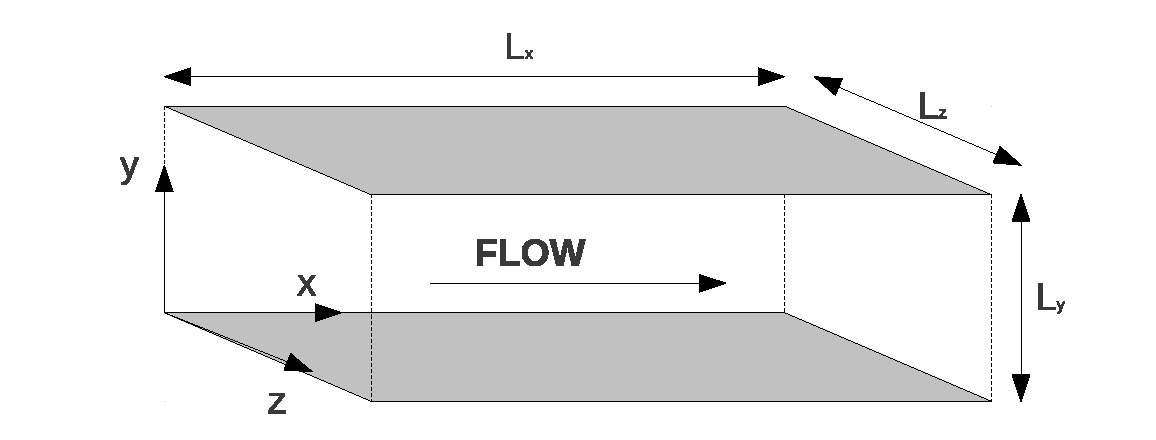
\includegraphics[width=0.8\linewidth]{dns_config.ps}
\caption{Channel flow geometry.}
\label{pic:configuration}
\end{figure}

%A dimensionless velocity or Reynolds number of
%$Re_\text{bulk} = 3300$, based on the mean centreline velocity and
%$Re_{\tau}=183$, based on the wall shear velocity were chosen which
%offers a good comparison to a previous to statistics obtained by
%\citet{kmm87} as well as some guidance in referrence to mesh design
%due to other studies. The applied mesh uses about 768\,000 grid
%points ($ 80 \times 120 \times 80 $ in $x$,\,$y$,\,$z$). Nevertheless, all
%essential scales of turbulence are resolved on the computational grid
%and no subgrid model is used. Figure \ref{pic:mesh} shows one of the
%80 $z$-planes of the used mesh. \

%=============================================================================
\section{Parameters}

To match \citet{kmm87} we will aim for a bulk flow Reynolds number
based on the centreline mean speed $U$ and channel half-height
$\delta=L_y/2$ of $\Rey_\delta=U\delta/\nu=3300$.  For this flow the
associated Reynolds number based on the friction velocity
$u_\tau=(\tau_w/\rho)^{1/2}$ and half-height is
$\Rey_\tau=u_\tau\delta/\nu=183$. (It is worth noting that the
relationship between the bulk and friction Reynolds numbers for
turbulent flows is empirically based. For channel flow, a reasonable
approximation is given by $\Rey_\delta/\Rey_\tau=2.5\ln\Rey_\tau+5$,
while for turbulent flow in a pipe of diameter $D$, Blasius'
correlation $\Rey_\tau=u_\tau D/2\nu=99.44\times10^{-3}\Rey_D^{7/8}$
is quite good at moderate Reynolds numbers.)

\citet{kmm87} used domain extents of $L_x=4\pi\delta$ and
$L_z=2\pi\delta$ but for illustrative purposes we will choose the
smaller sizes $L_x=2\pi\delta$ and $L_z=\pi\delta$. We will find that
the turbulence statistics examined are apparently little affected by
this reduction in domain size, but the cost of simulation is
significantly reduced.  Since we will use Fourier expansions in the
$z$ direction we will have the basic spanwise wavenumber
$\beta=2\pi/L_z=2$.  This is set below by the simulation token
\texttt{BETA = 2}.

We will choose second-order time integration, usually the best
compromise between stability and accuracy.  (This is set below by the
token \texttt{N\_TIME = 2}, which could actually be omitted from the
session file since that is the default value.)

We need to choose a spectral element polynomial order. Values around 9
provide a good compromise between speed and accuracy for this
code. This is set with the token \texttt{N\_P = 10} (the number of
points along the edge of an element, one more than the polynomial
order).  Sometimes in what follows we will also approximate the
typical number of mesh divisions along the the edge of an element as
10, although the sharp-eyed reader will note that it should logically
be 9.

We need to choose the kinematic viscosity, $\nu$. We aim to have
$\Rey_\delta=3300$. It is good simulation/numerical practice to aim
for a characteristic velocity scale of unity, as well as a
characteristic mesh length scale of unity. In this case these goals
imply that we aim for a centreline mean speed $U\simeq1$ and our
channel half-height $\delta=1$.  With these choices we are left with
\[
  \nu = \Rey_\delta^{-1} = 303 \times 10^{-6},
\]
which is set by the simulation token \texttt{KINVIS = 303e-6}.

When using periodicity in the streamwise direction, a body force is
required in order to maintain the flow.  This is needed because the
pressure as well as the velocity is required to be
streamwise-periodic. The required body force per unit mass
(i.e. acceleration) is calculated from a time-average force balance in
$x$-direction for the entire channel
\begin{eqnarray*}
 \rho \times f_x \times
  \underbrace{\cancel{L_x} \times L_y \times \cancel{L_z}}_{\text{channel
    volume}}  &=& 2 \times \tau_w \times \underbrace{\cancel{L_x} \times
    \cancel{L_z}}_{\text{one wall surface}} \\ 
   \rho \times f_x \times \delta & = & \tau_w\\
    \frac{f_x\delta}{U^2} & = & \left(\frac{u_\tau}{U}\right)^2 = 
    \left(\frac{\Rey_\tau}{\Rey_\delta}\right)^2
  \label{eq:force_balance}
\end{eqnarray*}
where $\tau_w$ is the time-average wall shear stress.  With $\rho =
\delta = U= 1$ and (from correlation/previous results)
$\Rey_\tau=183$, $\Rey_\delta=3300$, the required value is
\[
  f_x = 3.08 \times 10^{-3} .
\]
This will be set with the token \texttt{FFX = 3.08e-3}.  Note that if
required for body forces in the $y$ or $z$ directions there are
corresponding tokens \texttt{FFY} and \texttt{FFZ} respectively.
These body forces are added to the component momentum equations (the
\NavSto\ equations).  Also note that the code is written assuming
$\rho=1$.

The friction velocity $u_\tau=(\tau_w/\rho)^{1/2}\equiv
U\Rey_\tau/\Rey_\delta=55.5\times10^{-3}$, and the viscous wall length
scale $l_w=\nu/u_\tau=5.46\times10^{-3}$.

%============================================================================
\section{Mesh design}

In designing the mesh for the channel flow, rules of thumb established
in related studies \citep{pio97,kmm87,blsc03} have been
considered. All mentioned coordinates are with respect to coordinate
system established in this work. Thus, $x$ is the streamwise
direction, $y$ the wall-normal and $z$ the spanwise direction ---
Fourier expansions are always used in the $z$ direction.


\citet{kmm87} used $\Delta x^+ =\Delta x / l_w = 12$, $y^+ = 0.05$ (at
the wall) and $\Delta z^+ = 7$ in their study. \citep{pio97} proposed
similar values with $\Delta x^+ = 15$, $\Delta y^+ < 1|_\text{wall}$
and $\Delta z^+ = 6$.
%Referencing \citeauthor{pio97}, \citet{blsc03} used a mesh with
%$\Delta x^+ = 85$, $y^+ = 10$, $\Delta z^+ = 32$ for the individual
%element with $8 \times 8$ GLL nodes in $(x,y)$.

The wall-normal part of the spectral element mesh design strategy for
wall-resolved LES described by \citet{blsc03} is to terminate the
element closest to the wall at $y^+=10$, the second element at
$y^+\simeq35$, then use a geometric progression of sizes to reach the
flow centreline (one has to choose the number of elements and
geometric expansion factor).  This ensures there is good resolution in
the viscous-dominated wall layer as well as the buffer layer
($10<y^+<35$), where turbulent energy production is greatest.
Nevertheless, here, the second element layer is reduced to $y^+ = 25$
in order to improve resolution in the middle of the buffer layer.

The first two element heights in the wall-normal direction are then
$\Delta y_1(10)=0.056$ and $\Delta y_2(25)=0.139$. For the remainder,
we use a geometric progression of four elements starting with an
initial height of $\Delta y = 0.139-0.056=0.083$ to reach the channel
centreline.  The total number of elements in the $y$-direction is 12.

Next considering the $x$-direction, the indicative mesh spacing is
$\Delta x^+=15$, corresponding to a length $\Delta x =
15\times5.46\times10^{-3}=81.9\times10^{-3}$.  The number of grid
points needed to cover the domain extent in the $x$-direction is then
of order $N_x=2\pi/\Delta x=76.7$.  For a mesh with \verb|N_P=10| we
need of order 8 elements.  So our $(x,y)$ spectral element mesh is now
of size $8\times12=96$ elements.

Finally considering the $z$ direction, we have $L_z=\pi$ and want
$\Delta z^+\simeq7$, or $\Delta
z\simeq7\times5.46\times10^{-3}=38.2\times10^{-3}$.  The implied
number of $z$ planes is then of order $\pi/38.2\times10^{-3}=82.2$.
We need an integer number of planes which must be even (one prime
factor of 2) and other allowable prime factors of 3 and 5.  80 planes
seems convenient so we choose \verb|N_Z = 10|.  Note that means we
could run on either a single processor in serial execution or 2, 4, 8,
10, 20 or 40 in parallel.  There will be 40 Fourier modes.

%Figure \ref{pic:profile}(a) illustrates these rules in question and
%allows to compare them to the mesh ultimately used (b) showing the
%average streamwise velocity.
%\begin{figure}[b]
%\centering
%\subfigure[ ]
%{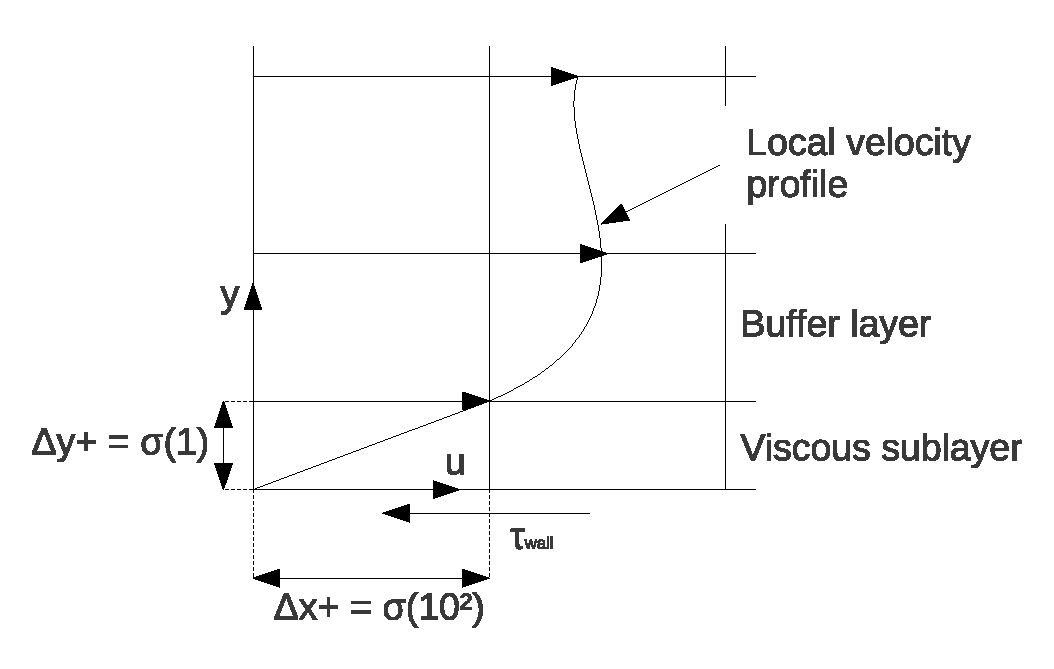
\includegraphics[height=50mm]{dns_profile.ps}}
%\subfigure[ ]
%{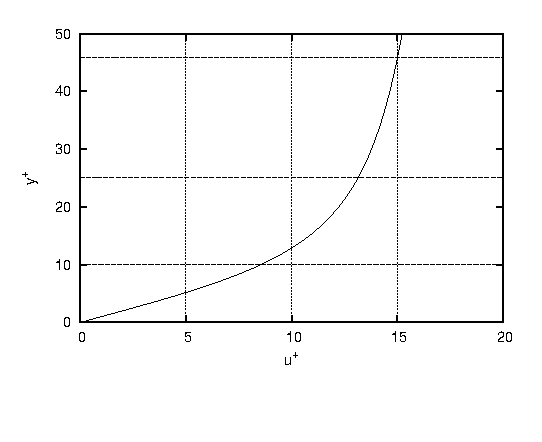
\includegraphics[height=50mm]{dns_wall_profile.ps}}
%\caption{Mesh design in the near wall region (a) and real distribution (b)}
%\label{pic:profile}
%\end{figure}

The mesh can be created using the provided tool \texttt{rectmesh}
which reads from an input file containing two blocks with all grid
lines in $x$ and $y$ separated by an empty line. The output from
running \verb|rectmesh| will be a valid \Semtex\ session file but which
will generally need some editing. 

{\small
\begin{verbatim}
rectmesh [options] mesh.inp > sessionfile
\end{verbatim}
}

A \verb|rectmesh| input file for this case is as follows: {\small
\begin{verbatim}
-3.14159265358979
-2.35619449019234
-1.5707963267949
-0.785398163397448
0.0000
0.785398163397448
1.5707963267949
2.35619449019234
3.14159265358979

-1.0
-0.944
-0.861
-0.745
-0.575
-0.330
0.0
0.330
0.575
0.745
0.861
0.944
1.0
\end{verbatim}
}

Once this file is built, all the above mentioned parameters can be
changed to their desired value. Also, the boundary conditions have to
be named and set into place.  We use wall boundary conditions on the
upper and lower edges of the domain, and edit the \verb|<SURFACES>|
section to obtain periodicity in the streamwise direction. Here the
example input file for this particular case:

{\small
\begin{verbatim}
################################################################
#  96 element channel flow, for Re_bulk = 3300, Re_tau = 183

<FIELDS>
	u v w p
</FIELDS>

<USER>
	u = 1.0-y*y
	v = 0.0
	w = 0.0
	p = 0.0
</USER>

<TOKENS>
	N_TIME = 2
	N_P    = 10
	N_Z    = 80
	BETA   = 2.0
	N_STEP = 60000
	D_T    = 0.002
	KINVIS = 303e-6
	FFX    = 3.08e-3
	IO_CFL = 100
	IO_HIS = 100
	AVERAGE = 2
</TOKENS>

<GROUPS NUMBER=1>
	1	w	wall
</GROUPS>

<BCS NUMBER=1>
	1	w	4
			<D> u = 0.0 </D>
			<D> v = 0.0 </D>
			<D> w = 0.0 </D>
			<H> p       </H>
</BCS>

<NODES NUMBER=117>
    1	       -3.14159             -1              0
  ...
  117	        3.14159              1              0
</NODES>

<ELEMENTS NUMBER=96>
    1	<Q>    1    2   11   10    </Q>
  ...
   96	<Q>  107  108  117  116    </Q>
</ELEMENTS>

<SURFACES NUMBER=28>
    1    1    1    <B> w </B>
    2    2    1    <B> w </B>
    3    3    1    <B> w </B>
    4    4    1    <B> w </B>
    5    5    1    <B> w </B>
    6    6    1    <B> w </B>
    7    7    1    <B> w </B>
    8    8    1    <B> w </B>
    9   89    3    <B> w </B>
   10   90    3    <B> w </B>
   11   91    3    <B> w </B>
   12   92    3    <B> w </B>
   13   93    3    <B> w </B>
   14   94    3    <B> w </B>
   15   95    3    <B> w </B>
   16   96    3    <B> w </B>
   17    8    2    <P>   1      4       </P>
   18   16    2    <P>   9      4       </P>
   19   24    2    <P>  17      4       </P>
   20   32    2    <P>  25      4       </P>
   21   40    2    <P>  33      4       </P>
   22   48    2    <P>  41      4       </P>
   23   56    2    <P>  49      4       </P>
   24   64    2    <P>  57      4       </P>
   25   72    2    <P>  65      4       </P>
   26   80    2    <P>  73      4       </P>
   27   88    2    <P>  81      4       </P>
   28   96    2    <P>  89      4       </P>
</SURFACES>

<HISTORY NUMBER=1>
	1	0.0	0.0	0.0
</HISTORY>
\end{verbatim}
}


%=============================================================================
\section{Initiating and monitoring transition}


The critical bulk Reynolds number for linear instability of channel
flow is $\Rey_c = 5772$ but turbulence can typically be maintained down
to lower values (and here we are aiming at $\Rey_\delta=3300$) if
transition is obtained. Our strategy here will be to start from a
laminar flow profile and add some white noise to obtain transition.
This is done using the following single line to generate an initial
condition: {\small
\begin{verbatim}
compare chan | noiz -p 0.1 chan.fld > chan.rst
\end{verbatim}
}

Here, the command-line value 0.1 represents the standard deviation of
the normal/Gaussian distribution from which the noise is derived using
a pseudorandom number generator and is therefore quite large compared
to an average velocity of $U=1$. It is necessary, since our Reynolds
number is here below the critical value, to assure a sufficient amount
of disturbance to initiate transition to a turbulent state. If the
Reynolds number were above the critical value, any perturbation level
above machine noise level should eventually produce transition --- it
just depends on how long you are prepared to wait. We note that
channel flow is a case for which it is relatively easy to obtain
transition to turbulence without carefully manipulating the noise
level, or restricting the time step.

In order to monitor transition, a very useful diagnostic is to monitor
the evolution of kinetic energies in all Fourier modes.  Transition
should be easy to see as a moderately rapid increase in turbulent
energy within small scales that are represented by higher wave
numbers. Figure~\ref{pic:modal_en}(a) shows the transition for the
mentioned channel flow. Figure~\ref{pic:modal_en}(b) indicates that
the resolution is adequate due to a separation of about three and a
half decades between the highest and smallest wave number. An increase
of energy within the highest wave numbers would also indicate an
under-representation because of aliasing of the energy of higher modes
back into the resolved frequency domain (which is the underlying
reason for the plateau seen at the highest wavenumbers in
figure~\ref{pic:modal_en}(b)).

\begin{figure}
   \centering
   \subfigure[ ]
   {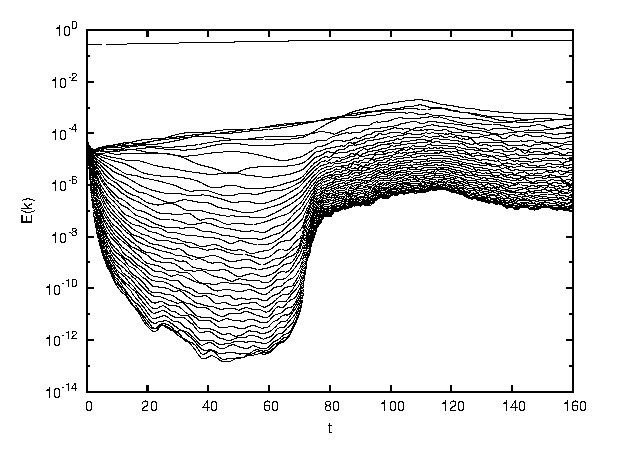
\includegraphics[height=0.22\textheight]{dns_modal_t.ps}}
    \subfigure[ ]
   {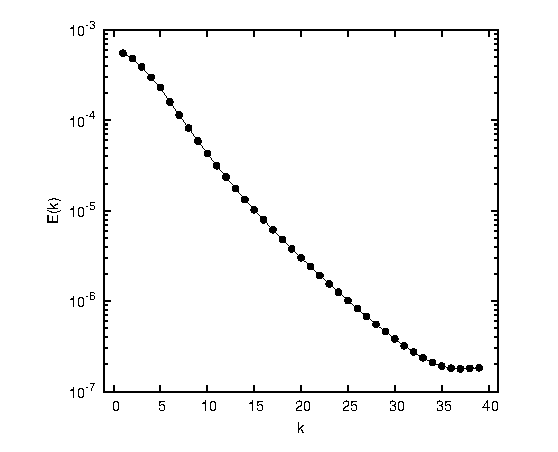
\includegraphics[height=0.22\textheight]{dns_modal_k.ps}}
    \caption{Modal energies for (a) the individual wave numbers over
      time and (b) by wavenumber.}
    \label{pic:modal_en}
\end{figure}

Figure~\ref{pic:modal_en}(a) shows the evolution of kinetic energies
in the 40 Fourier modes represented.  By way of interpretation, the
mode with highest energy (here, and typically) is mode~0, which
represents the \twod\ or $z$-average flow.  All the other modes start
off with much the same energy, which is a result of having chosen to
pollute all modes equally when using the \verb|noiz| utility (often,
one would just pollute mode~1 and allow convolution to distribute
energy to all other modes --- this gives a more gentle perturbation).
The highest modes typically decay rather rapidly initially, with the
lower modes either slowly losing or (as here, gaining) energy.  Also
the energy in mode~0 here increases a little over time, partly because
the initial condition here actually had a lower volumetric flow rate
than the equilibrium turbulent flow. At $t\approx70$ the flow makes a
transition to a turbulent state, typically signalled by the higher
modes gaining energy fairly rapidly until a quasi-equilibrium is
reached. Eventually the flow settles to a statistical equilibrium at
$t\approx140$.  Figure~\ref{pic:modal_en}(b) shows the temporal
average values of energies in the various Fourier modes.  (The
\SM\ macros \verb|moden| and \verb|modav| were used to
plot figure~\ref{pic:modal_en}.)

%=============================================================================
\section{Flow statistics}

Flow statistics can be collected by setting the \verb|AVERAGE| token
to non-zero values 1, 2 or 3 (here a value of 2 was used, see below).
See also \S\,\ref{sec.average}.  To obtain statistical convergence it
is necessary to average over a sufficiently long time, just as would
be the case in a physical experiment. Statistics are updated every
\verb|IO_HIS| simulation steps (here, every 100 steps).  In the
present case, the total averaging time was chosen to be 400, which
represents of order 60 `wash-through' times, since the domain length
is $2\pi$ and the bulk flow speed $U=1$.  Since the time between data
updates is $100\times0.002=0.2$ there are a total of $400/0.2=2000$
averaging buffer updates.

Once the simulation is run, a \texttt{.avg} file is produced. For
\verb|AVERAGE=1|, statistics for the represented fields are collected,
\ie $\langle u\rangle$, $\langle v\rangle$, \ldots, $\langle
p\rangle$.  For \verb|AVERAGE=2|, averages of velocity field products
are stored too, \ie $\langle uu\rangle$, $\langle uv\rangle$, etc.
For \verb|AVERAGE=3|, additional products are collected to allow
computation of terms in the fluctuating energy equation.  Note that it
is necessary to calculate Reynolds stresses and energy equation terms
in post-processing (\eg $\langle u'v'\rangle = \langle
uv\rangle-\langle u\rangle\langle v\rangle$).  Note also that if
\verb|.avg| files exist, they are read in at start of execution of
\verb|dns| to initiate averaging buffers: the \verb|Step| value in the
file's header stores the number of averages obtained to date.

Having collected statistics, our next step is to calculate the
Reynolds stresses and to average in $x$- and $z$-direction. To
illustrate the possible processing, here is an example shell script:

{\small
\begin{verbatim}
#!/bin/bash

# temporary files
FTNZ='/tmp/chan_nz1'
FTRS='/tmp/reynolds-stress.xy'
FRSY='./reynolds-stress.y'

# average field results in z
project -z1 chan.avg > /tmp/chan.avg.xy

# calculate reynolds-stresses (xy-plane)
rstress /tmp/chan.avg.xy > $FTRS

# new input file with NZ=1
LNZ=$(cat cube | grep N_Z -n | awk -F: '{print $1}')
sed '$LNZs/.*/  N_Z    = 1/' <chan >$FTNZ

# average reynolds-stresses in x
rayavg npts navg y_0 x_0   y_0 x_1 dy dx $FTNZ $FTRS >  $FRSY
rayavg npts navg y_0 x_1   y_0 x_2 dy dx $FTNZ $FTRS >> $FRSY
...
rayavg npts navg y_0 x_n-1 y_0 x_n dy dx $FTNZ $FTRS >> $FRSY

# PLOTTING
gnuplot ~/scripts/plot_rstress.gpl;
\end{verbatim}
}

Figure \ref{pic:u_wall} shows the mean velocity profile for the
channel flow in comparison to data from \citet{kmm87}. The dashed
lines are representing the linear respectively logarithmic part of the
law of the wall.  Figure \ref{pic:rms_global} show rms Reynolds stress
values in friction velocity units with comparison to data from
\citet{kmm87}.  Quite good agreement is evident.

\begin{figure}
\centering
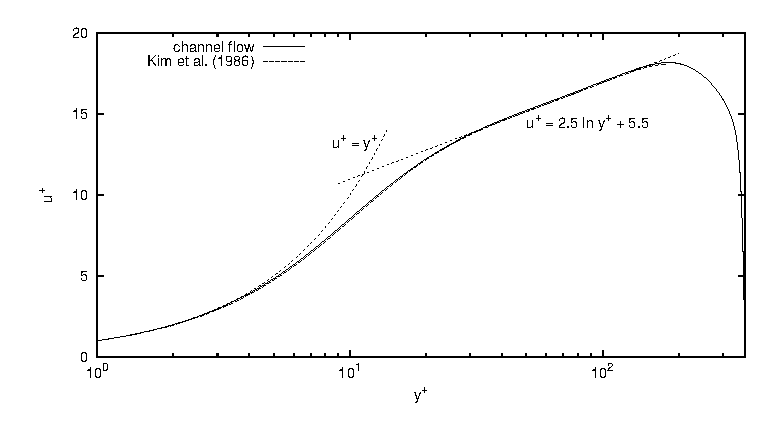
\includegraphics[width=0.7\linewidth]{dns_u_wall.ps}
\caption{Mean velocity profile of the channel flow compared to the law
  of the wall and data from \citet{kmm87}}
\label{pic:u_wall}
\end{figure}


\begin{figure}
\begin{center}
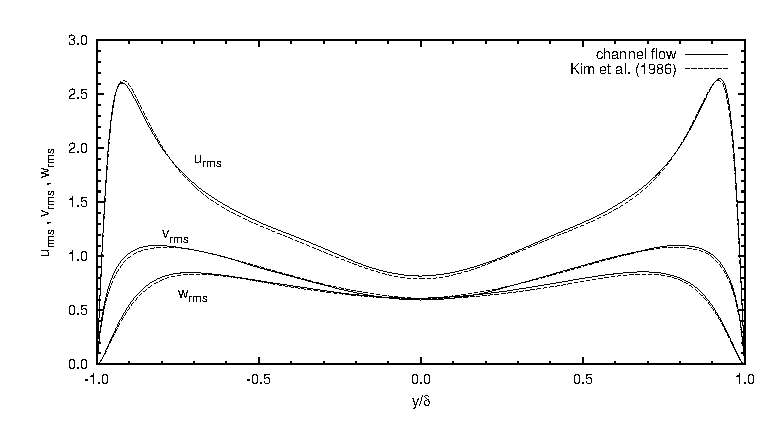
\includegraphics[width=0.7\linewidth]{dns_rms_global.ps}\\
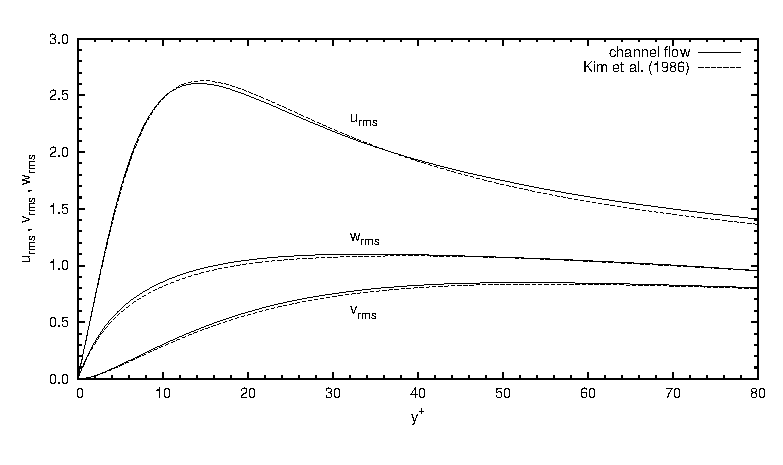
\includegraphics[width=0.67\linewidth]{dns_rms_wall.ps}
\end{center}
\caption{ Root-mean-squares velocity fluctuations in global
  coordinates normalized by the wall shear velocity
  $u_{\tau}$. Comparison to data from \citet{kmm87}.}
\label{pic:rms_global}
\end{figure}

%%%%%%%%%%%%%%%%%%%%%%%%%%%%%%%%%%%%%%%%%%%%%%%%%%%%%%%%%%%%%%%%%%%%%%%%%%%%%

\bibliographystyle{dcu}
\bibliography{userguide}

%%%%%%%%%%%%%%%%%%%%%%%%%%%%%%%%%%%%%%%%%%%%%%%%%%%%%%%%%%%%%%%%%%%%%%%%%%%%%
\end{document}
